% !TEX encoding = UTF-8 Unicode
% !TEX TS-program = pdflatex

%%%%%%% La riga soprastante serve per configurare gli editor
%%%%%%% TeXShop, TeXworks e TeXstudio per gestire questo file
%%%%%%% con la codifica UFF-8.
%%%%%%% Se si vuole usare un'altra codifica si veda sotto.
%%%%%%%

%%%%%%%  Esempio con molte opzioni
%%%%%%% Le opzioni nella forma "chiave=valore" sono definite
%%%%%%% perché la classe dalla versione 6.1.00 usa il pacchetto
%%%%%%% xkeyval. Vedere sulla documentazione in inglese o
%%%%%%% in italiano quali chiavi accettano valori.

%%%%%%% L'opzione per il corpo accetta qualsiasi valore, anche fratto
%%%%%%% (per esempio: corpo=11.5pt) e va sempre scritto con una
%%%%%%% unità di misura. L'utente è pregato di non esagerare con
%%%%%%% corpi normali minori di 9.5pt o maggiori di 13pt.
%%%%%%%
%%%%%%% Le opzioni per inputenc e fontenc vanno per prime.
%%%%%%% Vengono ignorate se NON si compone con pdfLaTeX. Ma
%%%%%%% questo è un esempio per pdfLaTeX.
%%%%%%%

\documentclass[%
corpo=12pt,
twoside,
stile=standard,
% oldstyle,
%    autoretitolo,
tipotesi=magistrale,
numerazioneromana,
% libro, utile per la stampa => mette il margine diverso per la rilegatura
greek,
evenboxes,
]{toptesi}
%%%%%%%%%%%%%%%%%%%%%%%%%%%%%%%%%%%%%%%%%%%%%%%%%%%%
%%%%%% Per la codifica d'entratasi può scegliere quella che si vuole,
%%%%%% ma si consiglia di preferire utf8; in ogni caso non scegliere
%%%%%% codifiche specifiche del sistema operativo.

\usepackage[utf8]{inputenc}% codifica d'entrata
\usepackage[T1]{fontenc}%    codifica dei font
\usepackage{lmodern}%        scelta dei font
% \usepackage[
% backend=biber,
% style=alphabetic,
% sorting=ynt
% ]{biblatex}
% \addbibresource{biblio.bib}
% Vedere la documentazione toptesi-it.pdf per le
% attenzioni che bisogna usare al fine di ottenere un file
% veramente conforme alle norme per l'archiviabilità.


\usepackage{hyperref}

\hypersetup{%
    pdfpagemode={UseOutlines},
    bookmarksopen,
    pdfstartview={FitH},
    colorlinks,
    linkcolor={blue},
    citecolor={blue},
    urlcolor={blue}
}
%
%%%%%%% Esempio di composizione di tesi di laurea con PDFLATEX 
%
%
% Per scrivere testo fasullo in "latinorum"
\usepackage{lipsum}
%

%%%%%%% Definizioni locali
\newtheorem{osservazione}{Osservazione}% Standard LaTeX
\ExtendCaptions{italian}{Abstract}{Acknowledgements}

\begin{document}\errorcontextlines=9
%%%%%%% Questi comandi è meglio metterli dentro l'ambiente
%%%%%%% ThesisTitlePage con o senza asterisco, oppure in un file di
%%%%%%% configurazione personale. Si veda la documentazione
%%%%%%% inglese o italiana.
%%%%%%% Comunque i presenti comandi servono per comporre la
%%%%%%% tesi con i moduli di estensione standard del pacchetto
%%%%%%% TOPtesi.

\begin{frontespizio*}
    % Per cambiare la dicitura sopra la lista dei laureandi decommentare
    % la riga seguente, cambiando le 4 parole in modo consistente
    %

    \TitoloListaCandidati{Studente,Studenti,Studentessa,Studentesse}
    %
    \ateneo{Politecnico di Torino}
    \logosede[150px]{polito_logo_2021_blu}% 

    %
    % Non tutte le università hanno un nome proprio
    % \nomeateneo{Sede di Torre sosjd}
    %
    % \struttura[III]{Matematica, Fisica e~Scienze Naturali}
    %\Materia{Remote sensing}
    
    \titolo{Anomaly detection per il rilevamento di attacchi DDoS su reti aziendali}% per la laurea quinquennale e il dottorato
    % \sottotitolo{Metodo dei satelliti medicei}% per la laurea quinquennale e il dottorato
    %
    %%%%%%% Corso degli studi
    \corsodilaurea{Ingegneria Informatica}% per la laurea
    
    %%%%%%% L'eventuale numero di matricola va fra parentesi quadre
    % \show\Candidato
    \def\Candidato{Candidato}
    %\show\Candidato
    \candidato{Stefano \textsc{Loscalzo}}[s267614] 
    %\secondocandidato{Evangelista \textsc{Torricelli}}[123457]
    
    %%%%%%% Relatori o supervisori
    %
    \relatore{prof.~Guido \textsc{Marchetto}}
    % \secondorelatore{dipl.~ing.~Werner von Braun}
    % \terzorelatore{dott.~Mario Rossi}
    % 
    %%%%%%% Per mettere altri relatori consultare toptesi-it.pdf
    
    %%%%%%% Tutore
    \tutoreaziendale{dott.\ ing.\ Francesco \textsc{Lucrezia}}
    \NomeTutoreAziendale{Supervisore aziendale\\Tiesse S.p.A.}
    
    %%%%%%% Seduta dell'esame
    %\sedutadilaurea{Agosto 1615}
    %%%%%%%% oppure:
    \sedutadilaurea{Anno~Accademico 2020-2021}% 
    
    %%%%%%% Logo della sede
\end{frontespizio*}


%%%%%%% Per cambiare l'offset per la rilegatura;
%%%%%%% meno offset c'e', meglio e'
%\setbindingcorrection{3mm}




%%%%%%% Questo test è usato appunto per collaudare diversi stili,
%%%%%%% non per comporre una vera tesi.
%%%%%%% Non usarlo mai, solo perché qui è usato!
\ifclassica%
{\begin{dedica}
Dedica qui
% \textdagger\ A non so
\end{dedica}
\fi
%%%%%%% Fine esperimento

% Si veda la documentazione per verificare la differenza fra abstract
% e summary. Perciò se se ne usa uno, non si deve usare l'altro.
\english
\begin{abstract}
This short abstract, is typeset with the \texttt{abstract} environment (from the \texttt{report} document class) just to test if it works. or what concerns working, it works, but in Italian ist title turns out to be ``Sommario'' in bold face series and normal size; its apperance looks like  a bad copy of what one obtains with the \texttt{\string\summary} command. In English, though, its title is “Abstract”, as it should be, since at the beginning of this template a suitable \texttt{\string\ExtendCapions} command was issued.

Please, read the documentation  in Italian (file \texttt{toptesi-it.pdf} in order to fully understand the difference beteesn “abstract” and “summary” in the context of this bundle.

\end{abstract}

% Fine dell'altro esperimento
\italiano
\sommario

Gli attacchi di denial of Service distribuiti (DDoS) sono uno dei maggiori problemi di sicurezza delle reti. Hanno lo scopo di impedire ad utenti legittimi l'accesso a dei servizi o degradare loro le prestazioni. In questa tesi proveremo a identificare anomalie riconducibili ad attacchi DDoS, in un contesto di una rete aziendale con più sedi, usando un riconoscimento delle anomalie effettuato tramite rete neurale allenata su dati provenienti dai router di più sedi aziendali e una successiva mitigazione degli attacchi tramite un agent sugli stessi. 

% \paginavuota % funziona anche senza specificare l'opzione classica
\italiano

% \tablespagetrue\figurespagetrue % normalmente questa riga non serve ed e' commentata
\indici


\mainmatter

\chapter{Introduzione}

\section{Motivazione}
% Spiegare il perché l'ho fatto Dati importanti, piccole e medie imprese devono sfruttare software opensource disponibili a tutti che permetto di passare da una frase experimental a production ready

Le piccole e medie imprese sono sempre più informatizzate e dipendenti da servizi informatici per poter svolgere il loro lavoro. Per questo motivo scoprire e analizzare il traffico anomalo in transito sulle reti aziendali è sempre più importante, il nostro obiettivo è farlo ad un basso costo, senza aggiungere hardware o applicativi che richiedano molta potenza di calcolo o di banda, sfruttando i router che compongono la rete. Punteremo a scoprire le anomalie nei dati di rete sui singoli flussi e nei dati aggregati analizzando alcune metriche su un server aggiuntivo che si occuperà anche di mitigare l'attacco informando i router sui flussi da bloccare o limitare.
Gli attacchi maggiormente presi in considerazione in questa tesi saranno gli attacchi di ``Distributed Denial of Service'', ma gli stessi principi potranno essere applicati anche ad altre tipologie di anomalie.
% problema delle botnets
Inoltre l'analisi dei dati raccolti sull'utilizzo della rete potrà portare anche alla risoluzioni di problemi di rete non derivanti da attacchi.

\section{Collaborazione con Tiesse s.p.a.}

Questa tesi è stata sviluppata in collaborazione con Tiesse s.p.a.: un'azienda che progetta e realizza, interamente in Italia, router e dispositivi M2M, con connettività wired e mobile.

L'azienda ha oltre 20 anni di esperienza, ed è stata riconosciuta come uno dei maggiori fornitori di CPE a banda larga e wireless su reti 3G/4G dalla maggior parte delle compagnie telefoniche. Oltre alla produzione e alla progettazione di router e apparecchiature di rete, sviluppa progetti custom, sia hardware che software. I prodotti Tiesse sono particolarmente adatti ad applicazioni Business e Mission Critical per il Corporate Networking.

L'azienda è sempre attiva sull'aspetto di ricerca e sviluppo, anche tramite collaborazioni con il Politecnico di Torino e in particolare negli ultimi anni ha messo il focus su soluzioni software per la sicurezza e l'analisi dei dati di rete.

La sede centrale dell'azienda si trova ad Ivrea, ma possiede anche sedi distaccate a Torino, Avezzano e Roma.

% Scrivo quello dell'abstractafd
% lavoro svolto in collaborazione e in parte in presenza presso l'azienda spa di Ivrea

% Sezione in cui parlo di cui fa Tiesse spa
% - presento azienda
% - location e sedi distaccate
% - parlare della collaborazione con il poli => sempre in collaborazione per ricerca e sviluppo in particolare negli ultimi anni con un focus sugli aspetti di sicurezza e analisi dati di rete e non solo hw => prendere spunto anche dal sito
% - prendere ispirazione dalla slide tiesse di itasec

\section{Scenario}
\begin{figure}[]
    \label{fig:scenario}
    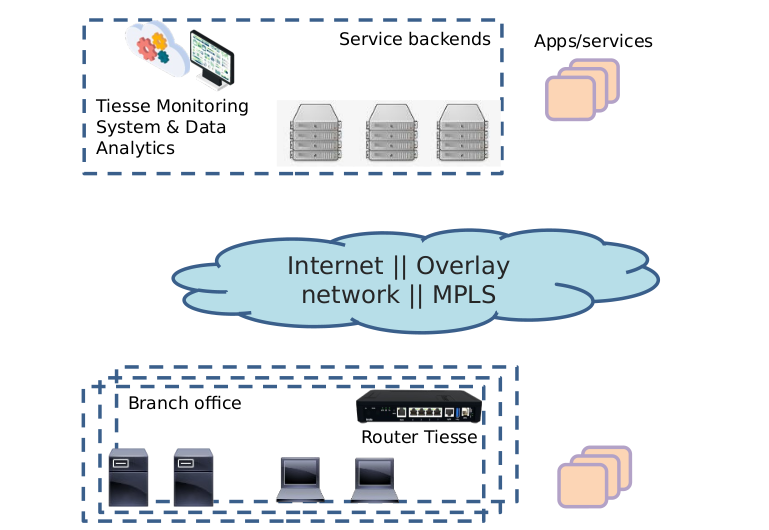
\includegraphics[width=\hsize]{images/introduzione/scenario_2.png}
    \caption{Scenario rete Tiesse e clienti}
    \centering
\end{figure}

Nello sviluppo della nostra soluzione abbiamo preso in considerazione un tipico scenario aziendale, in cui esiste una sede centrale, ben protetta e su cui sono ospitati i servizi dell'azienda e tante sedi periferiche: uffici, negozi o altro, collegati ai servizi della sede centrale tramite un overlay MPLS o una VPN.
Le sedi periferiche sono quelle più esposte sotto l'aspetto della sicurezza, \uline{anche solo per il fatto che sono in numero maggiore, spesso non ci sono i responsabili dell IT in sede e solitamente sono meno controllate rispetto la sede centrale}. Per questo motivo il nostro obiettivo è quello di proteggere i servizi, gli applicati aziendali e la rete centrale dai dispositivi malevoli connessi alle reti degli uffici.
L'organizzazione di Tiesse e di molti suoi clienti è caratterizzata dallo scenario in figura \ref{fig:scenario}. Utilizzando questa struttura di rete per effettuare la raccolta, l'analisi del traffico e le prove, ci siamo basati su un esempio di sede periferica, nel nostro caso un ufficio dell'azienda situato a Torino, con l'obiettivo di proteggere i servizi aziendali presenti nella sede centrale di Ivrea a cui l'ufficio è collegato tramite una VPN.

Un altro caso possibile di utilizzo di questa soluzione è la distribuzione dei servizi in cloud, in cui l'azienda non ha il controllo dell'infrastruttura di rete e sfrutta i router thrusted nelle reti degli uffici per analizzare il traffico.


% todo: sostituire servizi con applicativi aziendali

\begin{figure}[]
    \label{fig:scenario_2}
    %https://lucid.app/lucidchart/8119c7e9-e2e1-4dbb-b55f-bebf6c97af2d/edit?beaconFlowId=3612F8C43004D8D2&page=0_0#
    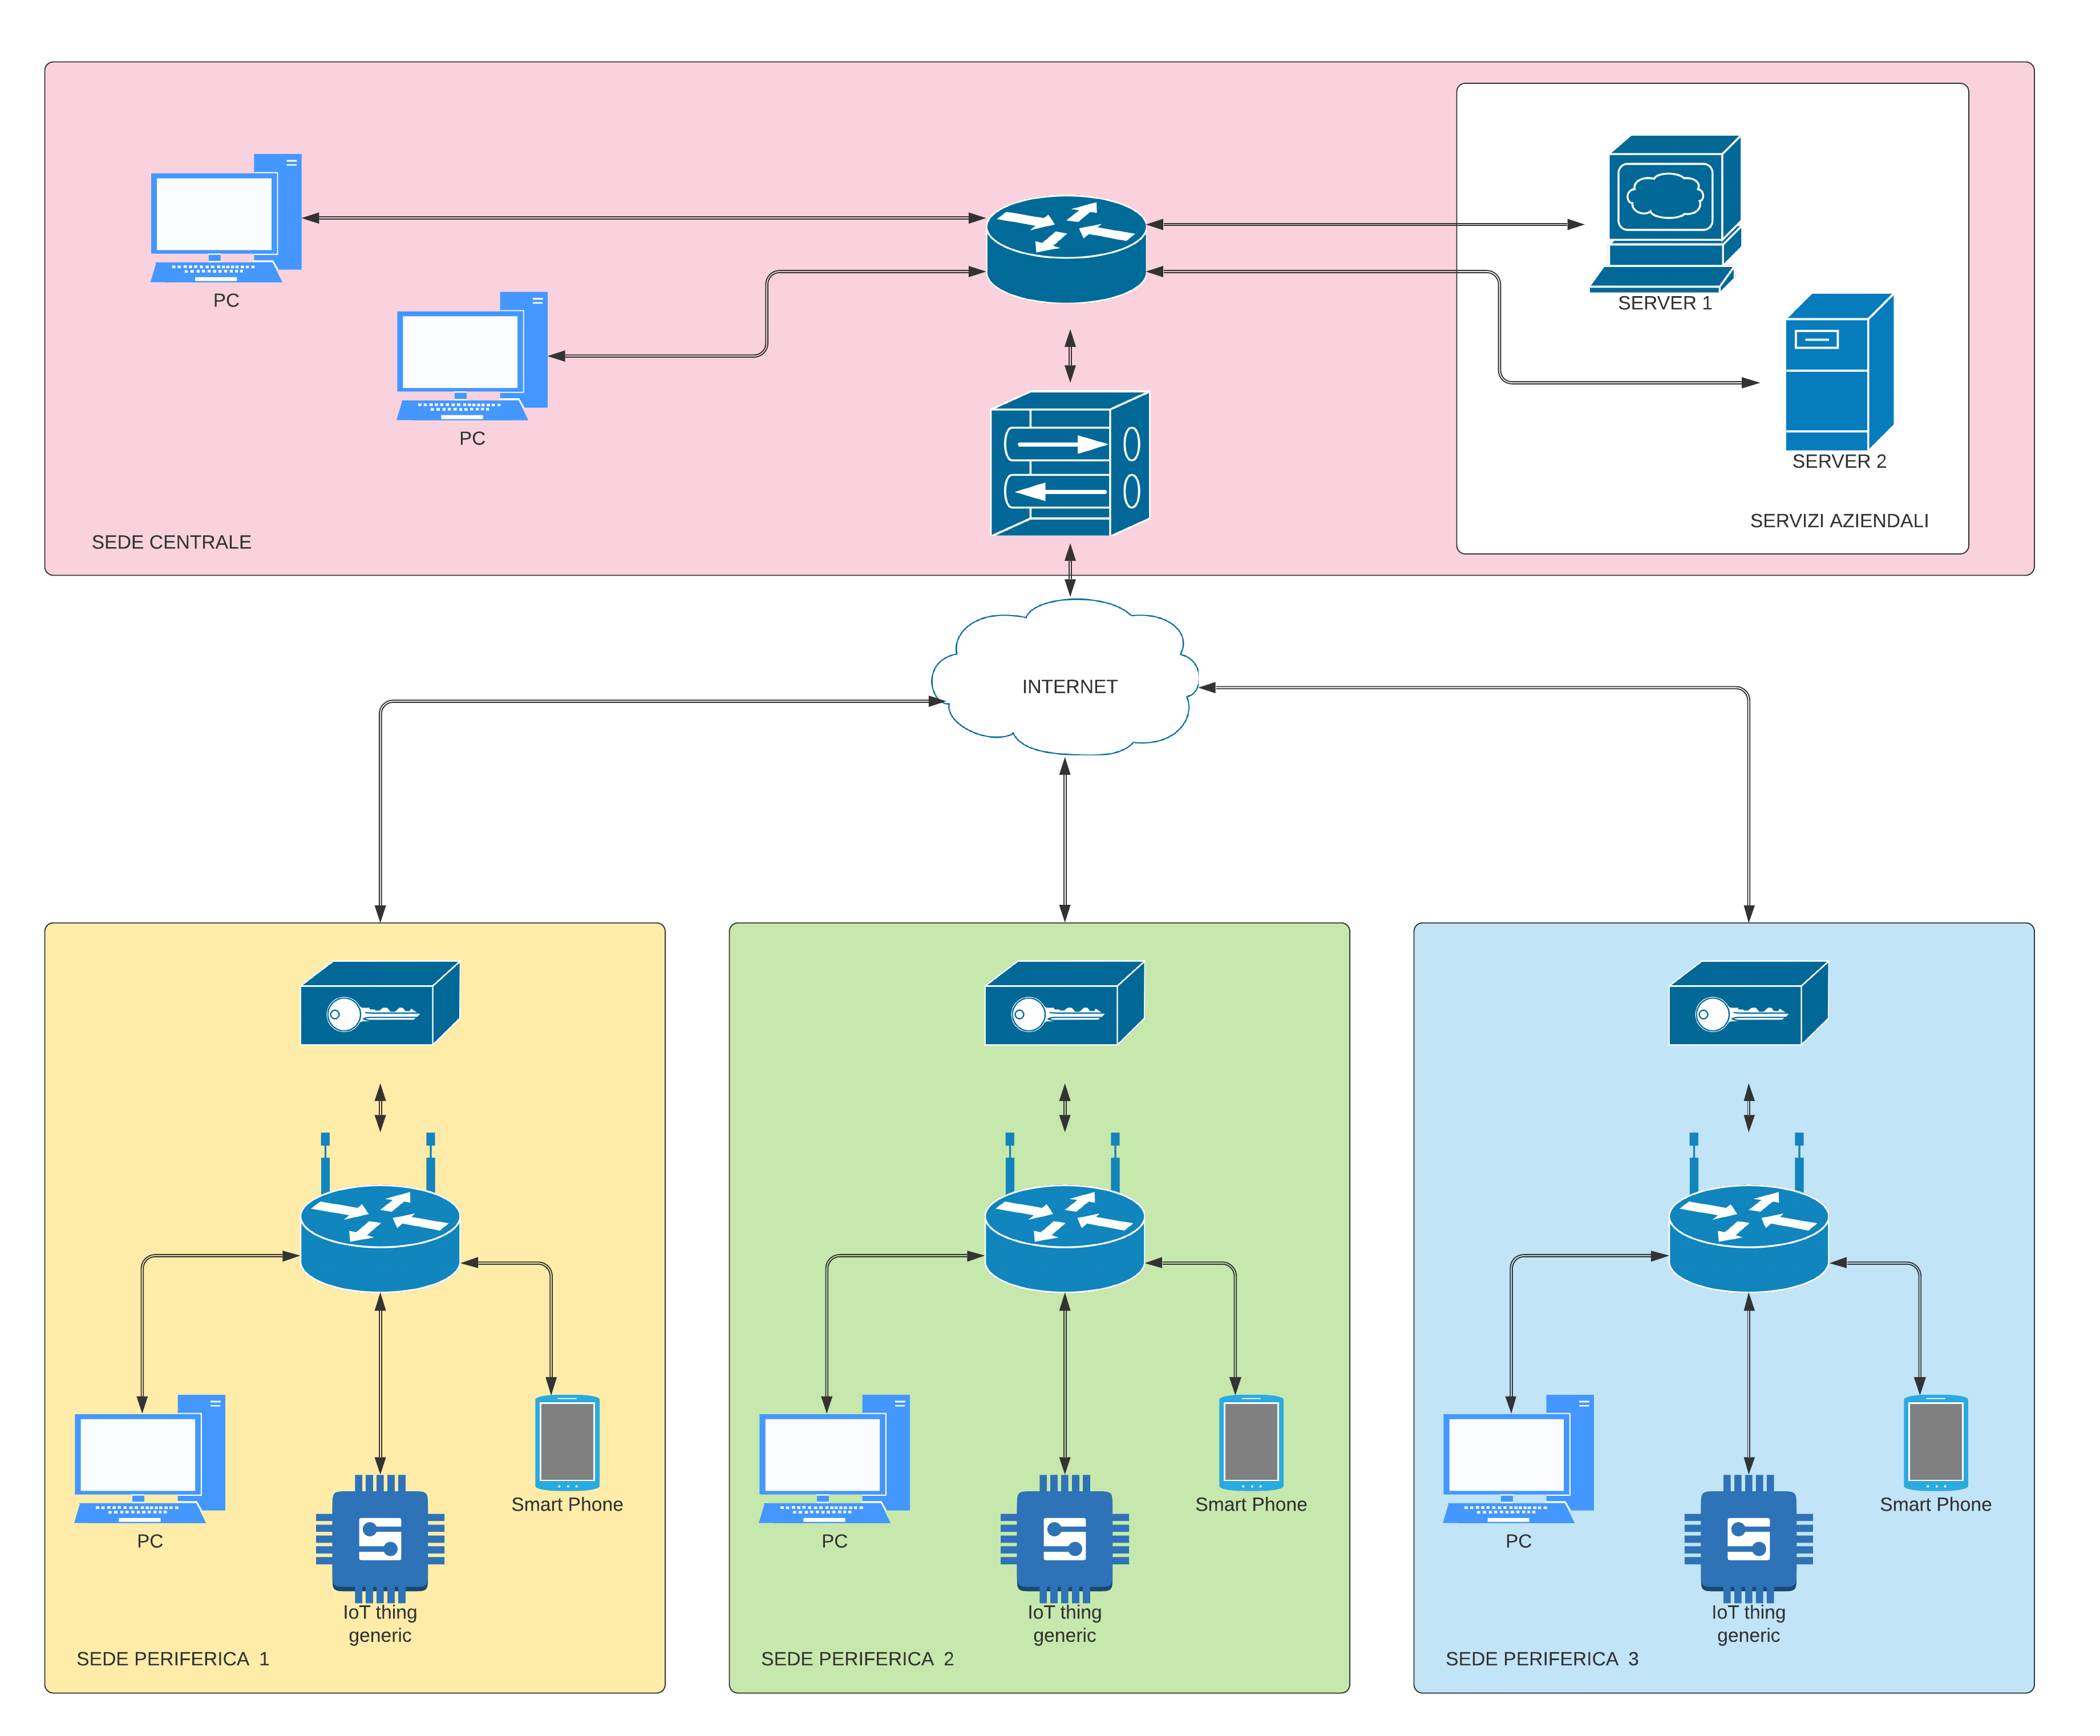
\includegraphics[width=\hsize]{images/introduzione/scenario.png}
    \caption{Scenario rete Tiesse e clienti}
    \centering
\end{figure}


\section{Gli attacchi DDoS}

Gli attacchi di Denial of Service (DoS) sono attacchi nel campo della sicurezza informatica che mirano a interrompere la fruizione di un servizio, fornito da un host connesso a internet, da parte di utenti legittimi. L'attacco ha l'obiettivo di esaurire le risorse dell'host in modo da non consentirgli di erogare le risposte ai richiedenti.
Nel caso in cui la sorgente del traffico che genera traffico malevolo per creare disservizi non sia unica, si parla di attacchi di denial of service distribuiti (Distributed Denial of Service).

\subsection{Tipologia di attacchi DDoS}
    
Gli attacchi DDoS possono essere suddivisi in due categorie principali in base al loro funzionamento. La prima si basa sul mandare alla vittima pacchetti malformati in grado di sfruttare un bug o una falla a livello applicativo. La seconda categoria invece si basa su tecniche utili a colpire l'infrastruttura del servizio, per il funzionamento di questa tecnica vengono usati uno o entrambi i seguenti metodi: il primo si basa sull'interruzione della connessione di rete grazie all'esaurimento della banda o della capacità di processamento dei router o di entrambe, nel secondo caso l'obiettivo dell'attaccante è di esaurire le risorse (es. sockets, CPU, memoria) del server che ospita il servizio \cite{ddos_survey_1}.

\begin{figure}[h]

    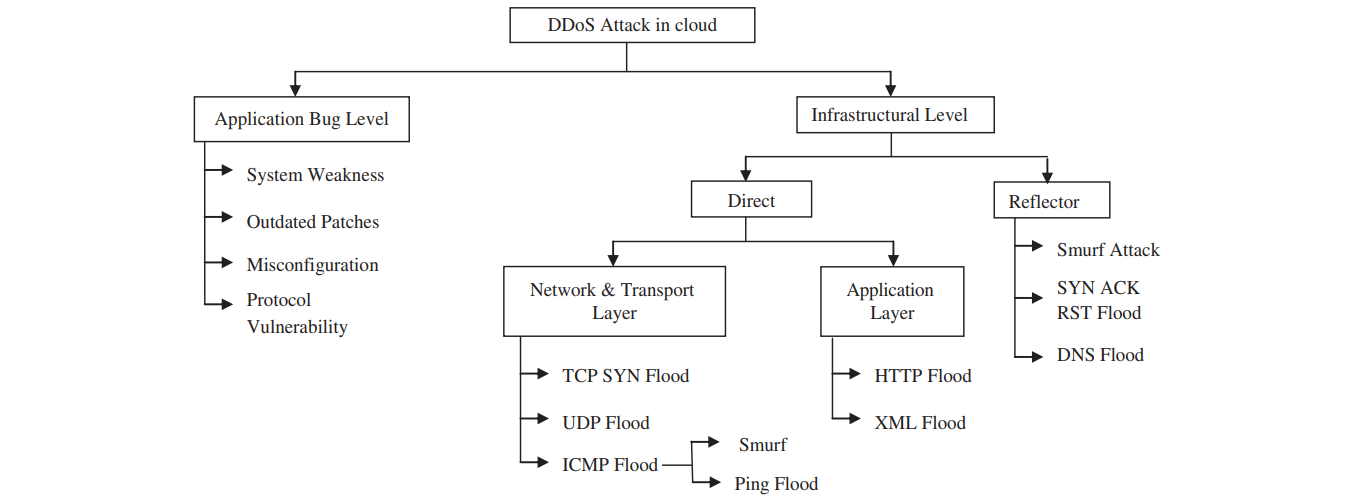
\includegraphics[width=\hsize]{images/introduzione/tipologie_ddos.png}
    \caption{Tipologie di attacchi DDoS \cite{ddos_survey_3}}
    \centering
\end{figure}

L'obiettivo di questa tesi sarà concentrato sul rilevamento e la mitigazione della seconda categoria di attacchi, basata sull'esaurimento delle risorse.

\subsubsection{Attacchi basati sul flooding}

\begin{figure}[h]
    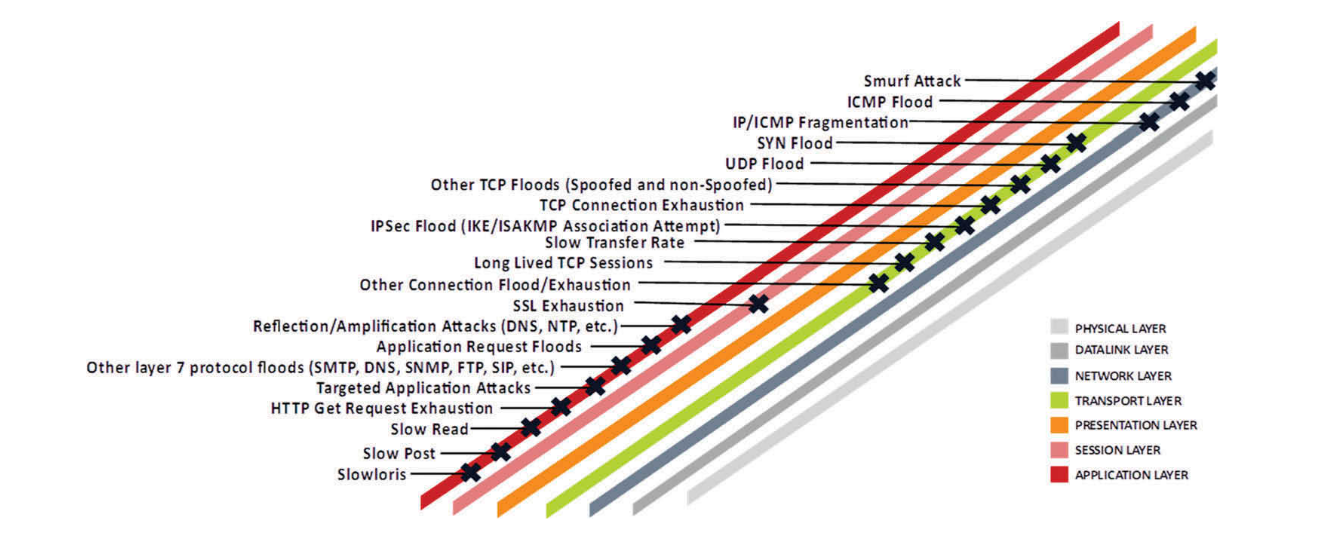
\includegraphics[width=\hsize]{images/introduzione/attacchi_per_livello.png}
    \caption{Attacchi per livello \cite{ddos_survey_4}}
    \centering
\end{figure}

\paragraph{Network/transport-level DDoS flooding attacks} % todo: rivedere titolo
Gli attacchi di denial of service che mirano ad esaurire le risorse di rete si basano sull'invio di molti pacchetti con lo scopo di consumare totalmente \uline{la banda o le socket} della vittima, queste tipologia di attacco può essere effettuata in maniera diretta: \emph{flooding attacks} e \emph{protocol exploitation attacks}, nel primo caso la vittima viene inondata di pacchetti (UDP flood, ICMP flood, DNS flood, VoIP flood an etc.), in questo caso la banda aggregata in uscita di tutti gli attaccanti deve essere superiore a quella del servizio che si vuole danneggiare, nel secondo caso vengono sfruttane delle caratteristiche dei protocolli della vittima in modo da consumare una grande quantità di risorse (es. TCP SYN flood, TCP SYN-ACK flood, RST/FIN flood e ecc).

Gli attacchi che non vengono effettuati in maniera diretta invece sfruttano la riflessione o l'amplificazione: nei \emph{Reflection-based flooding attacks} chi attacca manda un particolare pacchetto, indirizzandolo ad un riflettore e questo riflettore manda le sue risposte alla vittima, in modo da esaurirne le risorse. Un esempio di questa tipologia di attacchi sono lo Smurf e il Fraggle, nel primo vengono mandati ICMP Echo Request ad una sottorete, usando come ip di destinazione l'indirizzo broadcast e specificando come ip sorgente l'ip della vittima, utilizzando l'ip spoofing, causando la risposta di tutti gli host verso l'indirizzo della vittima \cite{ddos_survey_2}.
Gli \emph{Amplification-based flooding attacks} sfruttano servizi che restituiscono risposte più grandi della richiesta ricevuta, un esempio è il DNS amplification, che riesce a moltiplicare dalle 30 alle 50 volte\cite{imperva_amplification} la banda in uscita dell'attaccante, il suo funzionamento si basa sull'utilizzo dell'ip spoofing mandando un pacchetto con indirizzo ip sorgente della vittima, così il servizio DNS risponderà ad essa con un flood di pacchetti di dimensioni maggiori \cite{ddos_survey_1}. Lo stesso principio è sfruttato anche dal NTP amplification che può aumentare il traffico con un rapporto tra 20:1 e 200:1, arrivando in alcuni casi anche a 556:1 \cite{imperva_amplification}. 

% todo: Amplification-based flooding attack, negli attacchi di rete: qua non so giustificarla bene pagina 3 \cite{ddos_survey_1}
% qua parla bene del fattore di moltiplicazione degli attacchi https://www.imperva.com/blog/ntp-flood-explained/

\paragraph{Application-level DDoS flooding attacks} % todo: rivedere titolo
% qua taglio un po' corto sugli attacchi applicativi perché approfondirò maggiormente quelli di rete
Gli attacchi DDoS al livello applicativo hanno lo scopo di terminare le risorse del server(cpu, memory, disk/db bandwidth, I/O bandwidth),  solitamente usano meno banda rispetto gli attacchi rivolti verso l'infrastruttura di rete rete, per questo motivo è anche più difficile identificarli. Le tecniche utilizzate sono simili alle precedenti. Degli esempi sono l'HTTP flooding che effettuando l'invio di molte richieste HTTP, obbliga il server a produrre risposte che possono essere computazionalmente pesanti, oppure possono sfruttare l'SQL Injection per imporre un lock sul database e bloccare il funzionamento dell'applicazione. Altri attacchi di questa tipologia possono essere l'HTTP fragmentation, lo slowpost attack, slowreading attack e lo slowloris attack, tutte tecniche che mirano a mantenere molte connessioni aperte mandando o ricevendo pochi dati per volta \cite{ddos_survey_1}.
Gli attacchi di tipo applicativo sono molto eterogenei e non possono essere mitigati a livello di rete/trasporto, per questo motivo questa tesi prenderà in considerazione solo gli attacchi trattati al paragrafo precedente.

\paragraph{DDoS con obiettivo la riduzione della qualità del servizio}
\label{paragraph:ddos_degradation}
% parlare anche di attacchi a basso rate, ma da molte fonti che portano ad un grande risultato finale \cite{ddos_survey_4,ddos_survey_3} pagina 38, rendendolo difficile da indentificare

L'unico obiettivo possibile degli attacchi DDoS non è la sola interruzione del servizio, ma un altro risultato attuabile è la degradazione del servizio, consumando una parte di risorse destinate agli utenti legittimi e creando loro ritardi nelle risposte. Questo risultato può essere raggiunto utilizzando dei packet rate più bassi, e di conseguenza meno rilevabili o dei l'invio d flood di pacchetti con rate variabili \cite{ddos_survey_3, ddos_survey_4}.
Gli approcci a bassi rate sono utilizzati frequentemente dagli attacchi DDoS a larga scala, poichè l'aggregazione di moltissime fonti a basso rate portano comunque ad un grande risultato finale.

\subsection{Vittime attacchi DDoS}

% todo: introduzione: qua potrei nominare delle statistiche sugli attacchi con la distribuzione delle vittime
\begin{figure}[h]
    % todo: capire come gestire citazioni immagini a livello di copyright
    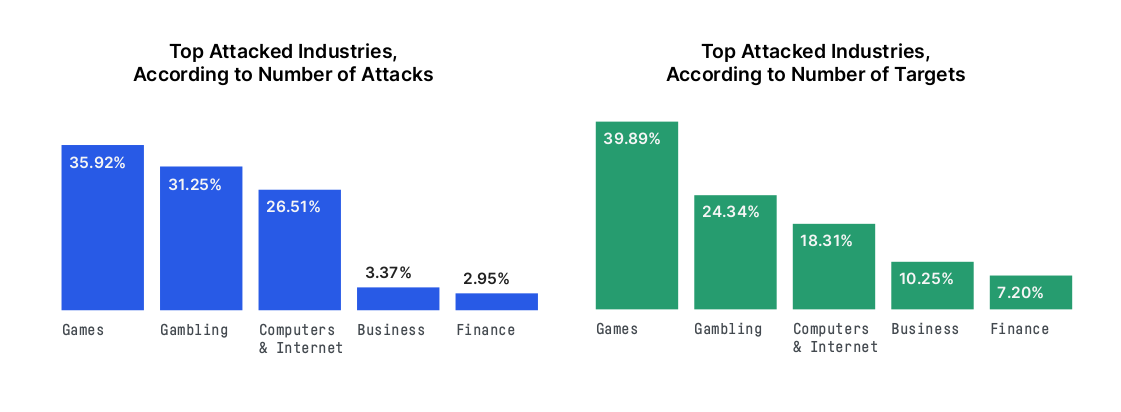
\includegraphics[width=\hsize]{images/introduzione/bersagli_ddos.png}
    \caption{Distribuzione vittime DDoS, 2020 \cite{imperva_ddos_report}}
    \centering
\end{figure}

I target degli attacchi DDoS possono differenziarsi molto: da un utente domestico ad un governo \cite{ddos_motivations}. Per capire maggiormente chi possono essere le vittime di un attacco bisogna analizzare le motivazioni che spingono gli attaccanti e con le diverse motivazioni si può anche capire qual'è il rischio per quanto riguarda la portata dell'attacco. 

Per semplicità possiamo suddividere gli incentivi di un attacco in cinque principali categorie \cite{ddos_survey_1, ddos_motivations}:

\begin{itemize}
    \item Beneficio economico o finanziario: sono gli attacchi riguardanti principalmente le aziende, sono considerati i più pericolosi e difficili da fermare. Mirano ad ottenere benefici finanziari dagli attacchi e i creatori dell'attacco sono abitualmente persone con esperienza.
    \item Vendetta: questa tipologia di attacchi sono mesi in atto da persone, solitamente con uno scarso livello tecnico, a fronte di un'apparente ingiustizia percepita.
    \item Credo ideologico: alcuni attaccanti si trovano ad effettuare attacchi contro alcuni obiettivi per motivi ideologici. È una motivazione di attacco meno comune delle altre, ma può portare ad attacchi di grande entità. % todo: valutare se mettere esempi attacchi tipo cnn 2008, wikileaks 2010 e iran 2009
    \item Sfida intellettuale: gli utenti che sviluppano attacchi per questa motivazione vogliono imparare e sperimentare a lanciarli. Spesso sono giovani appassionati di hacking che grazie alla facilità con cui si possono affittare botnets o utilizzare semplici tool riescono ad effettuare con successo DDoS.
    \item Cyberwarfare: gli attaccanti di questa categoria appartengono ad organizzazioni terroristiche o militari di un paese e sono politicamente motivati ad attaccare risorse critiche di un altro paese. Un grande numero di risorse viene usato per questa tipologia di attacco e può paralizzare le infrastrutture critiche di un paese, portando ad un grave impatto economico.
\end{itemize}


Le maggiori vittime secondo il report \cite{imperva_ddos_report} sono le compagnie che operano del campo dei videogiochi e delle scommesse, entrambe comportano un grande livello di rischio e spesso i giocatori si rifiutano di seguire le regole. Le aziende che incentrano il loro business sul settore di Internet e della computazione si trovano al terzo posto, seguiti dalle attività commerciali e da quelle finanziarie.


\subsection{Diffusione attacchi DDoS}


\begin{figure}[h]
    % todo: capire come gestire citazioni immagini a livello di copyright
    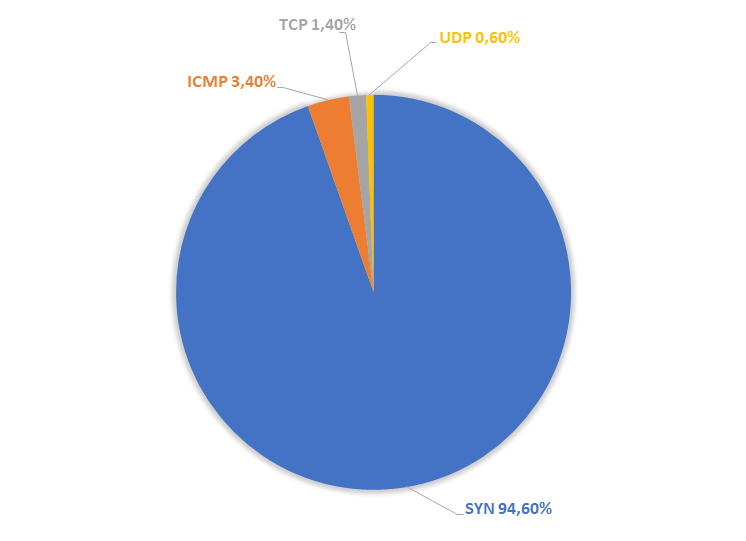
\includegraphics[width=\hsize]{images/introduzione/tesi_distribuzione_tipologia_attacchi.png}
    \caption{Distribuzione di attacchi DDoS per tipologia, Q3 2020 \cite{ddos_kaspersky_q3_2020}}
    \centering
\end{figure}

Nel mondo a fine 2020 la quasi totalità degli attacchi DDoS proviene da botnets, con target principali in Cina e negli Stati Uniti. Le tipologie di attacco maggiormente utilizzate sono il \emph{Syn Flood} che copre più del 90\% della totalità degli attacchi, seguito da \emph{ICMP flooding} e \emph{UDP flooding} \cite{ddos_kaspersky, ddos_kaspersky_q3_2020}.


La maggior parte degli attacchi DDoS hanno una portata inferiore ai 10 Gbps (circa il 65\%), ma il 3\% di essessi raggiunge cifre incredibili, superiori al 200 Mbps \cite{imperva_ddos_report}.

\begin{figure}[h]
    % todo: capire come gestire citazioni immagini a livello di copyright
    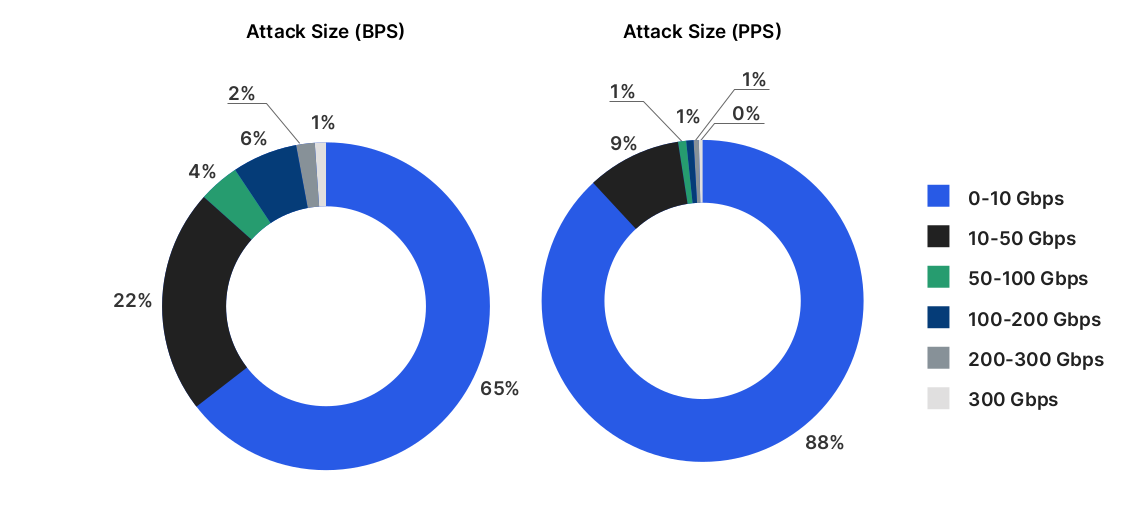
\includegraphics[width=\hsize]{images/introduzione/attacks_size.png}
    \caption{Distribuzione di attacchi DDoS per dimensione, 2020 \cite{imperva_ddos_report}}
    \centering
\end{figure}


\subsubsection{Attacchi basati su botnets}

Gli attacchi basati su botnets sono un grande problema per l'implementazione di sistemi anti-DDoS perché un grande numero di ``zombie'' rende l'attacco più distruttivo, in aggiunta spesso utilizzano ip spoofing complicando il tracciamento all'indietro per determinare la vera locazione bot \cite{ddos_survey_1}.

Il funzionamento delle botnet si basa su tre fasi. La prima consiste nel reclutamento ``dell'esercito'': fase in cui vengono contagiati i dispositivi tramite worms (programmi che si autopropagano) che sfruttano falle nella sicurezza. Sono usate tecniche come: la scansione automatica di indirizzi ip casuali per trovare altri soggetti vulnerabili, questa tipologia di scansione però produce molto traffico e può rendere possibile rilevare l'attacco, oppure una hitlist: una tecnica che frutta una lista di possibili macchine potenzialmente vulnerabili, la scansione della subnet o l'utilizzo di informazioni dei target basandosi sulle informazioni contenute nelle vittime infettate dai worm.


% todo: qui dovrei magari differenziare le botnet controllate direttamente e indirettamente e dilungarmi meno, magari nominare le tre fasi degli attacchi \cite{ddos_motivations} pagina 5 \cite{ddos_survey_4} pagina 37
Nella fase successiva alla creazione di un ``esercito'' avviene la propagazione delle informazioni riguardanti le vittime da attaccare, con la durata e l'ora.
I bot possono essere controllati dell'artefice dell'attacco tramite tre architetture \cite{ddos_survey_4}: % pagina 46
\begin{itemize}
    \item IRC-based: architettura client-server in cui ad ogni server si possono collegare centinaia di dispositivi, utilizza un protocollo testuale e utilizzando porte non standard rendendo molto difficile il riconoscimento del comando per lanciare un DDoS, il quale si può nascondere facilmente nel grande traffico dei server IRC. Il singolo server a cui si connettono tutti i client può essere considerato un single point of failure.
    \item Web based: ogni bot scarica periodicamente delle informazioni tramite una richiesta web ad un server, i comandi di questa tipologia di controllo sono i più difficili da tracciare.
    \item P2P based: le moderne botnet utilizzano una struttura più robusta e flessibile, invece di avere un singolo server centrale al controllo della botnet, viene mandato un comando in broadcast a tutti gli agent. Questo le rende più affidabili, poiché l'eliminazione di un agent non rende la rete non funzionante, ma al tempo stesso rende il mantenimento della rete più difficile e la scoperta di un agent può rivelare tutti gli altri. 
\end{itemize}
L'ultima fase è il tentativo di attacco vero e proprio.

\begin{figure}[h]
    % todo: capire come gestire citazioni immagini a livello di copyright
    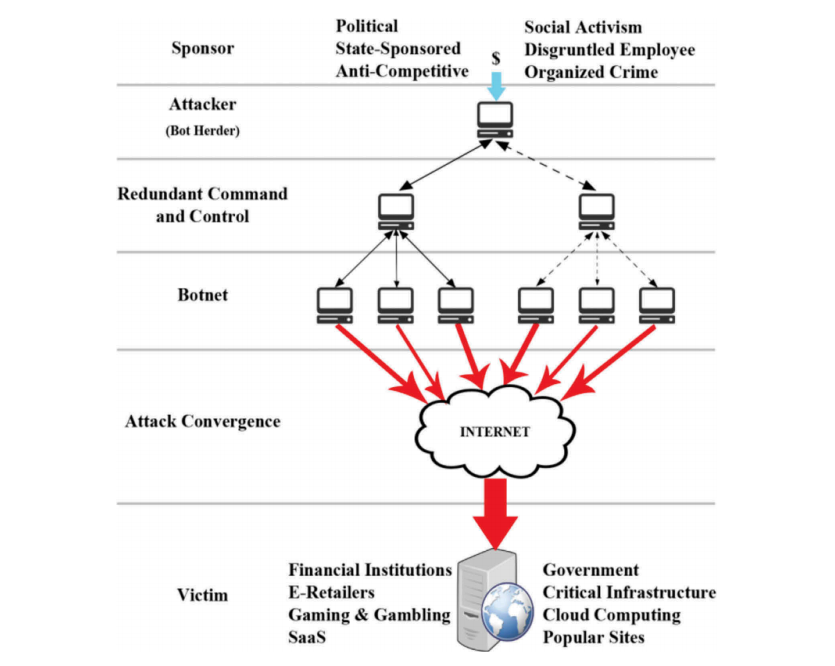
\includegraphics[width=\hsize]{images/introduzione/struttura_botnets_2.png}
    \caption{Struttura di lancio di attacchi DDoS \cite{ddos_survey_4}.}
    \centering
\end{figure}

Un esempio di botnet è Mirai, una rete di dispositivi creata attraverso un malware che sfrutta le vulnerabilità dei dispositivi IoT per creare host malevoli da utilizzare in attacchi DDoS di larga scala. Il codice sorgente del bot è stato rilasciato pubblicamente nel 2016, questo ha permesso la creazione di molte sue varianti, lasciando a chiunque la possibilità  di crearsi la propria botnet.
Il codice per effettuare attacchi DDoS include dieci tipologie diverse di attacco, ognuna configurabile in molti modi e lanciabile attraverso l'utilizzo di un server di comando e controllo \cite{slide_mirai}.

Alcuni attacchi possibili tramite la botnet Mirai sono: flood DNS, STOMP: una attacco che mira ad effettuare il three-way TCP handshake e solo dopo quando la sessione sarà messa in whitelist inizia un ACK flood, GREIP: incapsula nel pacchetto GRE un pacchetto ip con ip sorgente e destinazioni casuali, SYN flood, ACK flood, UDP flood e HTTP flood.

\subsubsection{Attacchi DDoS famosi}

%todo: qua parla del flood dns https://www.cloudflare.com/it-it/learning/ddos/dns-flood-ddos-attack/

Aggiungo questa parte o sarebbe superflua?

Potrei parlare dei primi attacchi, fino a quelli moderni menzionando i motivi dell'attacco se scoperti, la tipologia e la portata.


\section{Organizzazione della tesi}

La tesi nei successivi capitoli tratterà lo stato dell'arte dei sistemi anti-ddos esistenti (capitolo 2), mostrando come è possibile riconoscere un attacco e dove è meglio farlo per poterlo mitigare al meglio. Nel capitolo 3 approfondirà maggiormente lo stato dell'arte dei sistemi di anomaly detection da utilizzare per rilevare un attacco DDoS.
Nei capitoli 4 e 5 verrà illustrata la soluzione da noi proposta, focalizzandosi nel quarto sulla tecnica per rilevare un'anomalia e nel quinto su come mitigarla.
Nel capitolo 6 vengono menzionati possibili lavori futuri e nel 7 le conclusioni con delle considerazioni sulla soluzione proposta.
\chapter{Stato dell'arte}

\section{Riconoscimento DDoS}

\section{Contromisure attacchi DDoS}

\subsection{Soluzioni alla sorgente}

\subsection{Soluzioni alla destinazione}

\subsection{Soluzioni distribuite}

\chapter{Anomaly Detecion: stato dell'arte}

\section{Cos'è l'anomaly detection?}


L'anomaly detection si riferisce al problema di trovare pattern nei dati che non sono conformi al comportamento aspettato. A queste non conformità ci si riferisce come anomalie \cite{anomaly_detection_survey_3}. L'importanza del rilevamento delle anomalie è il fatto che un'anomalia nei dati spesso corrisponde ad un'informazione critica nel dominio a cui si riferisce, per esempio nelle reti di computer un traffico anomalo potrebbe significare che un computer è stato hackerato e sta compiendo azioni per il danneggiamento dell'azienda.

\section{Sfide dell'anomaly detection}

Le anomalie sono definite come un pattern che non rispetta il normale comportamento, ma il definire il concetto di normalità è una sfida, i maggiori fattori che influiscono su questa decisione sono \cite{anomaly_detection_survey_3}:

\begin{itemize}
    \item La difficoltà nel trovare una regione che comprenda tutti i possibili comportamenti normali è molto difficile e il confine tra azioni normali e anomale spesso non è ben definito.
    \item Se le azioni anomale sono generate da azioni malevole, il responsabile cercherà di fare in modo che le osservazioni sui dati appaiano normali.
    \item In alcuni contesti il comportamento si evolve e ciò che è considerato correntemente normale potrebbe essere rappresentativo per il futuro.
    \item È difficile definire quanto la differenza dalla normalità debba essere considerata anomala, per esempio in medicina piccole variazioni della temperatura corporea possono essere considerate anormali, in finanza la fluttuazione del valore delle azioni potrebbe essere considerato normale.
    \item La disponibilità di dati già classificati come normali o anomali per verificare il modello è uno dei problemi principali.
    \item Spesso i dati contengono rumore che tende ad essere simile alle anomalie ed è difficile rimuoverlo o distinguerlo.
\end{itemize}

\subsection{Stazionarietà dei dati}
Per dati stazionari si intende quando le proprietà statistiche dei dati non si evolvono nel tempo, questo non significa che i dati puntuali non variano, ma che il valore medio e la varianza rimangono costanti. Questa condizione sarebbe ideale per i nostri meccanismi di anomaly detection, ma è difficilmente attuabile in un contesto reale, in cui sono presenti dei trend e i dati potrebbero essere soggetti ad una stagionalità.

\section{Sistemi di rilevamento delle anomalie}

\subsection{Modalità di apprendimento}

% Abnormal in test data and most likely used as a
% specific type of the supervised techniques. Nearest neighbor
% techniques utilize the similarity or distance between samples to
% detect the anomalous data. Clustering techniques group the data
% to detect the individo}

I sistemi di anomaly detection necessitano di dataset con esempi di traffico per capire quando devono segnalare un'anomalia. In base alla tipologia di dataset di cui hanno bisogno per effettuare l'apprendimento, i sistemi di anomaly detection possono essere classificati in tre modi.

\paragraph{Apprendimento superivisionato}

I sistemi di anomaly detection basati su apprendimento supervisionato hanno prestazioni superiori ai metodi non supervisionati, poiché usano esempi etichettati di dati. I metodi supervisionati imparano il limite di separazione da un set di dati annotato durante una fase di allenamento e successivamente classifica le istanze da testare basandosi sul modello imparato. Avendo bisogno di etichette di difficile reperibilità, questo metodo è poco usato rispetto a quello semi-supervisionato e a quello non supervisionato, ma ha come vantaggi oltre al fatto di essere più preciso anche la velocità della fase di test, basandosi su un modello pre calcolato.
% Le tipologie di reti c
% Deep supervised techniques fail to separate normal from anomalous data if the feature space is highly complex and non-linear.

\paragraph{Apprendimento semi-superivisionato}

L'apprendimento semi-supervisionato è una tecnica che che per funzionare assume che tutti i dati usati per l'allenamento siano etichettati in un'unica classe, quella della normalità. Tutte le istanze di dati di dati di test che superano un certo limite intorno alla normalità verranno etichettate come anomale. I vantaggi di questo metodo è che l'uso di dati etichettati può portare ad un grosso miglioramento di performance rispetto alle tecniche non supervisionate, ma rischiano di non essere rappresentative di alcuni casi e sono inclini all'overfitting.
% qua la frase precedente non ha molto senso

\paragraph{Apprendimento non superivisionato}

Questa tecnica si basa su un set di dati normali che contengono che contengono una piccola quantità di dati anomali, l'algoritmo i occuperà di creare un punteggio di separazione basandosi su proprietà intrinseche dei dati.
%magari aggiungere altro pagina 23 \cite{anomaly_detection_survey_2_deep_learning}


\subsection{Metodi di detection}

Una volta classificati i sistemi di anomaly detection in base al metodo di apprendimento, possono essere ulteriormente suddivisi in sei sottocategorie basate sulla tecnica di rilevamento \cite{anomaly_detection_survey_1_network, anomaly_detection_classification}.


\begin{figure}[]
    \begin{center}
    \label{fig:anomaly_classification}
    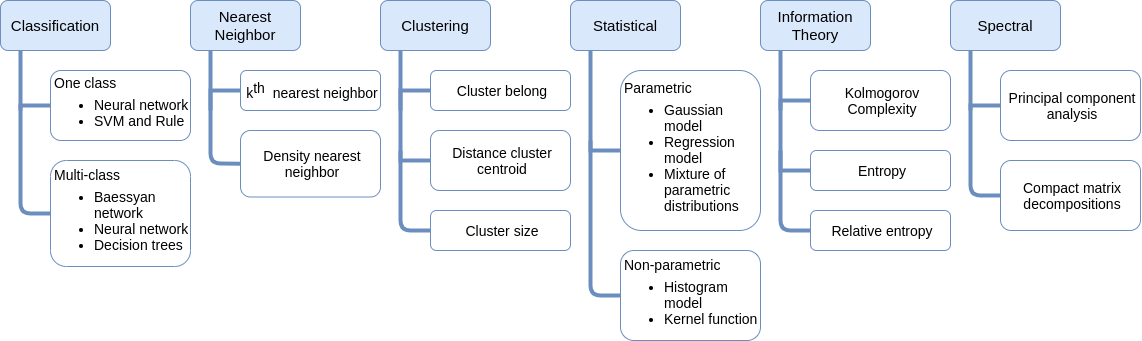
\includegraphics[width=\hsize]{images/reti_neurali/metodi_detection.png}
    \caption{Classificazione metodi di anomaly detection}
    \centering
    \end{center}
\end{figure}

% \cite{anomaly_detection_survey_1_network} pagina 24
\begin{itemize}
    \item Classification based: si basano su un set di dati etichettato che distingue una o più categorie e si basa su un modello (classificatore) che impara a distinguere le classi durante la fase di allenamento.
    \item Statistical based: assumono che i dati normali si presentino con una maggiore probabili rispetto a quelli anomali e segnalano come anomali regioni di dati a bassa probabilità.
    \item Information theory: analizzano il contenuto dei dati per verificare se sono presenti irregolarità.
    \item Nearest neighbor: si basa sull'assunzione che i dati normali si concentrino in zone dense e le anomalie si presentino lontano da queste zone.
    \item Clustering-based: raggruppano le istanze di dati simili in gruppi, i dati che non appartengono a nessun gruppo sono considerati anomali.
    \item Spectral: trasferisce i dati in un sottospazio con minore dimensionalità in modo che le istanze anomale siano significativamente differenti.
\end{itemize}


% \subsection{Dati in input}
% pagina 6 \cite{anomaly_detection_survey_3}

\subsection{Output of Anomaly Detection}

Un'importante caratteristica è come sono rappresentate le anomalie in uscita dal modello, esistono due metodi: le etichette, tecnica con la quale i dati vengono etichettati con una categoria, tendenzialmente binaria per esempio possiamo etichettare i dati come normali o anomali. L'altro metodo è l'uso di un ``anomaly score'': un punteggio per ogni istanza di dati, che indica quando si discosta dalla normalità, imponendo delle soglie possiamo verificare quali dati sono anomali \cite{anomaly_detection_survey_1_network, anomaly_detection_survey_2_deep_learning, anomaly_detection_survey_3}.


\section{Classificazione delle anomalie}

\subsection{Tipologia di anomalie}
Un aspetto importante dell'anomaly detection è l'analisi delle anomalie che possono presentarsi, di conseguenza le anomalie possono essere classificate nel seguente modo:
\begin{itemize}
    \item Anomalie puntuali: un singolo dato che si discosta dalla normalità. Questo è il caso più semplice e su cui si concentra la maggior parte delle ricerche sui dati anomali. Un esempio è un utente che tutti i giorni scarica 1GB di dati quando arriva in ufficio, ma un giorno ne scarica 10.
    \item Anomalie contestuali: quando un insieme di dati si comporta in modo anomalo in un determinato contesto, per esempio il numero di acquisti su un sito durante il periodo di Natale è più alto che durante il resto dell'anno.
    \item Anomalie collettive: quando un'istanza di dati è anormale rispetto all'intero dataset, in questo caso i dati in sè non sono anomali, ma lo diventano quando presi insieme, un esempio è l'elettrocardiogramma, in cui se ci sono bassi valori per un lungo periodo possono identificare un problema.
\end{itemize}

\subsection{Applicazione anomaly detection}
% \subsection{Tipologie anomaly detection}

Le applicazioni dell'anomaly detection possono essere molteplici, qui un breve elenco delle possibili applicazioni \cite{anomaly_detection_survey_3}:

\begin{itemize}
%todo: dire per ogni tipologia di applicazione quale sistema per l'anomaly detection è usato: esempio nids autoencoders, va, o altro 

    \item Fraud detection: sono sistemi con lo scopo di riconoscere frodi, i occupano di rilevare attività illegali in diversi campi come quella assicurativo, finanziario e telefonico.
    \item Medical and Public Health Anomaly Detection: lavorano sui dati dei pazienti, che possono avere anomalie per diverse ragioni: errori di registrazione, errori degli strumenti di misura o una condizione anormale delle condizioni del paziente. Questi sistemi mirano a riconoscere anomalie puntuali usando sistemi semi supervisionati.
    \item Industrial Damage Detection: i dispositivi industriali sono soggetti ad usura e danneggiamenti, sistemi di anomaly detection applicati in queste situazioni possono permettere di prevenire o rilevare in anticipo questi problemi.
    \item Image Processing: permette di riconoscere anomalie significative in immagini durante il tempo (motion detection) o regioni anomale in immagini statiche.
    \item Anomaly Detection in Text Data: questi sistemi riconoscono principalmente gli argomenti o gli eventi in una collezione di documenti, le anomalie sono causate da nuovi eventi interessanti o argomenti anomali.
    \item Sensor Networks: anomalie nei rilevamenti dei sensori possono significare un difetto o un'intrusione.
    \item Intrusion detection systems(IDS): sono dei sistemi che puntano ad identificare attività malevole nei sistemi informativi, gli IDS possono essere installati su un computer, in quel caso si parla di ``Host Intrusion Detection (HIDS)'' oppure su una rete, in quel caso si parla di ``Network Intrusion Detection (NIDS)'', gli IDS possono essere signature-based oppure anomaly based, nel primo caso non si è in grado di riconoscere nuove tipologie di attacchi. In questo contesto vengono analizzate le anomalie collettive e sono preferiti sistemi di apprendimento semi-supervionato o non supervisionato, perché le etichette per i dati anomali non sono quasi mai disponibili. In questa tesi mi concentrerò sull'analisi di anomalie di rete basandomi su sistemi di anomaly detection. 
\end{itemize}

\subsection{Tipologia degli attacchi di rete}
%parlare di Network IDS E Host IDS pagina 9 \cite{anomaly_detection_survey_2_deep_learning}
Lo scopo della sicurezza di rete è di proteggere la confidenzialità, l'integrità e di assicurare la disponibilità delle risorse, quindi una minaccia viene definita come qualunque cosa cosa che ha caratteristiche finalizzate a compromettere la rete \cite{anomaly_detection_survey_1_network}. Un elenco di possibili minacce è:

\begin{itemize}
    \item Denial of service (DoS)
    \item Probe: viene sondata la rete per ottenere informazione sulla struttura della rete target o degli host, principalmente per scopi di ricognizione.
    \item User to root (U2R): è una tipologia di attacco, quando l'attaccante ha l'obiettivo di ottenere illegalmente accesso ad un account amministrativo per manipolare o fare uso illecito di risorse.
    \item Remote to user (R2U): è un attacco in cui l'attaccante  ottenere l'accesso di una macchina target, in modo di avere il privilegio di utilizzare la sua rete.
\end{itemize}

\section{Le reti neurali}

% Spiego cosa sono le reti neurali, come funzionano e come vengono allenate.
\subsection{Funzionamento delle reti neurali}

Le reti neurali sono composte da diversi strati (layer) di nodi, ciascuno collegato al successivo.

L'unità base di ogni rete neurale è il nodo, che rappresenta il neurone artificiale, il tipo base è il ``perceptron'': un nodo con più input e un output rappresentato come una funzione a gradino caratterizzata dalla funzione ~\ref{eq:perceptron}, in cui si può notare che solo se la sommatoria dei valori in ingresso supera una certa soglia, il neurone si attiva.
\[
\label{eq:perceptron}
output = \begin{cases}
    0 & \mbox{if } \sum_{j}{w_{j}x_{j}}\leq \mbox{threshold} \\
    1 &  \mbox{if } \sum_{j}{w_{j}x_{j}} > \mbox{threshold}
\end{cases}
\]
Questo permette di compiere decisioni in base all'input.
%todo: Per esempio qui posso inserire l'esempio di pagina 3 del libro sulle reti neurali.

\begin{figure}[h]
    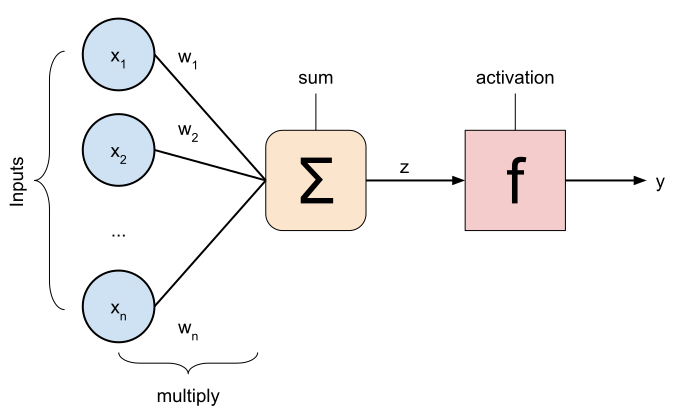
\includegraphics[width=300px]{images/reti_neurali/neurone.png}
    \label{fig:neurone}
    \caption{Neurone artificiale}
    \centering
    % https://www.doc.ic.ac.uk/~nuric/teaching/imperial-college-machine-learning-neural-networks.html
\end{figure}

Come si può notare dalla figura con l'evoluzione delle reti neurali non viene più usata solo la funzione a gradino, ma anche delle generiche funzioni rappresentate come ``f''.
Un esempio comunemente usato di evoluzione del perceptron sono i neuroni di Sigmoid, i quali invece di ritornare una funzione a gradino in uscita, ritornano il risultato della funzione di sigmoid ~\ref{eq:sigmoid} \cite{reti_neurali_libro}.

\begin{equation}
    \label{eq:sigmoid}
    \sigma(z) = \frac{1}{1+\mbox{exp}(-\sum_{j}{w_{j}x_{j}} - b)}
\end{equation}
\begin{figure}[h]
    \centering
    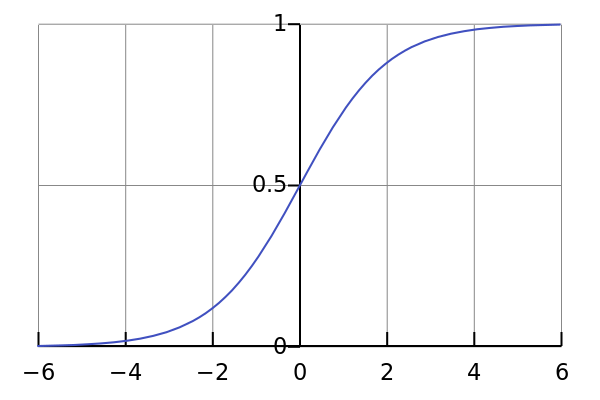
\includegraphics[width=200px]{images/reti_neurali/sigmoid-curve.png}
    \label{fig:sigmoid_curve}
    \caption{Esempio di curva di Sigmoid}
\end{figure}
Le reti neurali sono composte da gruppi di neuroni artificiali organizzati in livelli e tipicamente composte da almeno tre strati: uno di input, uno o più livelli intermedi definiti ``livelli nascosti'' e un livello di uscita. Ogni livello può contenere uno o più neuroni che possono essere collegati tra loro solo con dei collegamenti in direzione dai nodi di input a quelli di output, in questo caso si parla di ``feedforward'' oppure ``recurrent'' in cui sono previste delle connessioni di feedback a neuroni dello stesso livello o a livelli precedenti.
% 
%https://www.spindox.it/it/blog/ml1-reti-neurali-demistificate/
% fonte immagine https://towardsdatascience.com/what-the-hell-is-perceptron-626217814f53

\paragraph{Allenamento reti neurali}

L'allenamento di una rete neurale avviene ripetendo un percorso ciclico di tre fasi:

Il dataset in ingresso viene suddiviso in più gruppi, chiamati batch, e ogni elemento dei gruppi viene analizzato tramite la rete neurale, la quale calcolerà un valore. Calcolando la distanza tra il valore in uscita e il risultato corretto è 
possibile fare alcune modifiche ai pesi di ogni livello utilizzando l'algoritmo di retropropagazione dell'errore per avvicinare leggermente la predizione verso la risposta corretta \cite{reti_neurali_libro}. 
Questi passi verranno ripetuti più volte fino a quando non sarà ottenuto il risultato sperato.

\subsection{Autoencoders}
\begin{figure}[h]
    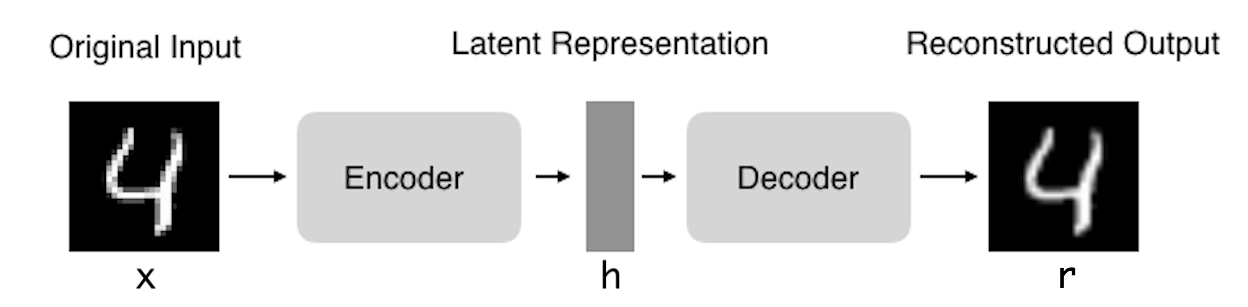
\includegraphics[width=\hsize]{images/reti_neurali/autoencoder.png}
    \caption{Struttura di un autoencoder}
    \label{fig:autoencoder}
    \centering
\end{figure}

%tate of a supercomputer node (lookingat the measured features); afterwards, the model can be used to no-tice representation changes that underlie anomalous conditions. Thishappens because an autoencoder is a neural network trained to copyits input푥to its output푦. Internally it has hidden layersℎencodingthe representation of the data. An autoencoder is composed by twosubparts: an encoding functionℎ=푓(푥)and a decoding function thatreconstructs the input푦=푔(ℎ). Typically, autoencoders do not simplylearn the identity function푔(푓(푥)) =푥but are designed not to beable to copy perfectly, thus the output of an autoencoder is generallydifferent from its input; this difference is calledreconstruction error. Thereconstruction error is used to identify anomalies. During training, anautoencoder learns the relationships among the features in the inputset. If new, previously unseen, data is given to the trained autoencoder
%todo: citare questo articolo https://www-sciencedirect-com.ezproxy.biblio.polito.it/science/article/pii/S0952197619301721

%To reduce overfitting, aDropoutlayer was applied (Srivastava et al.,2014) to the output of layers 1 and 2 (dropout rate equal to 0.2).

% Cosa sono gli autoencoder e perché sono utili nell'anomaly detection.

Gli autoencoder sono una tipologia di reti neurali non supervisionata, anche se quasi sempre vengono usati in maniera semi-supervisionata, che permettono di generare nuovi dati, effettuando in uscita la ricostruzione dei dati forniti in ingresso.
Gli autoencoder sono composti da tre parti, l'encoder, lo spazio latente e il decoder, negli autoencoder la dimensione dell'input è uguale a quella dell'output, e nel mezzo ci sono dei livelli che si occupano prima di comprimere (encoder) le dimensioni, fino a raggiungere lo spazio latente, una forma ``compressa'' dell'input, seguita da una serie di livelli (decoder) che si occupano di ritornare alle dimensioni originarie (Figura ~\ref{fig:autoencoder}).
La capacità di comprimere i dati e decomprimerli si basa sull'allenamento della rete, di conseguenza ogni rete è specifica per una tipologia di dati da comprimere e decomprimere, questo la caratterizza dagli altri sistemi di compressione, per esempio gzip, inoltre è una tipologia di compressione ``lossy'', con perdita, perché l'uscita sarà simile all'ingresso, ma degradata.
Una popolare applicazione degli autoencoder è l'anomaly detection. Gli autoencoder si occupano di ricostruire i dati iniziali, imparando effettivamente a riprodurre una funzione identità, per questo motivo allenandoli solo con dati di istanze normali quando si troveranno davanti ad un dato anomalo falliranno la ricostruzione dell'input e di conseguenza produrranno un grande errore di ricostruzione \cite{anomaly_detection_survey_2_deep_learning}. 
% https://towardsdatascience.com/applied-deep-learning-part-3-autoencoders-1c083af4d798#f686
% https://www.deeplearningitalia.com/introduzione-agli-autoencoder/


\section{Soluzioni esistenti di Anomaly Detection}

Esistono in letteratura sistemi di anomaly detection basati su autoencoders, che possono essere allenati per il riconoscimento di anomalie di rete basandosi su correlazioni non lineari tra le features, degli esempi sono:

\begin{itemize}
\item Kitsune \cite{kitsune}: un NIDS, basato sistema di anomaly detection basato su autoencoders, che permette il riconoscimento di traffico normale e anomalo senza una supervisione per l'allenamento. Il sistema ha l'obiettivo di rilevare attacchi di tipo DDoS, Man in the Middle, scansioni di rete e botnet in una rete con dispositivi tradizionali e IoT.
\item La soluzione proposta nell'articolo \citetitle{chen_autoencoders} \cite{chen_autoencoders} sfrutta una rete di autoencoders convoluzionaria (per una riduzione dei tempi di training) per superare le prestazioni dei sistemi di rilevamento tradizionali.
\item L'obiettivo della soluzione \cite{vae_autoencoders} è di rilevare attacchi in di rete utilizzando i dati provenienti dai router di rete, generati tramite NetFlow, inoltre si pone l'obiettivo di spiegare in cosa consiste l'anomalia nei dati. Per il rilevamento delle anomalie si basa sui Variational Autoencoder, uno sviluppo della versione tradizionale.


\end{itemize}

\section{Motivazione scelte}

% todo: da motivare le scelte per l'anomaly detection
% Perché autoencoders
% Quali sono i vantaggi rispetto ad altre soluzioni:

% - parlo del fatto che sfruttiamo le api messe a disposizione di keras e tensorflow perché sono facili da usare, ci sono soluzioni alternative da citare (tool di twitter scritto in R => informarsi)
% - gli autoencoders si prestano bene nel caso in cui non sappiamo a priori definire delle features astratte => ci basiamo solo sulla forma e non sul contenuto => non cerchiamo feature particolari per determinati  pattern https://blog.keras.io/building-autoencoders-in-keras.html
% - le forme possono cambiare da cliente a clientee
% - facili da usare, si passa velocemente da una fase experimental a prodution grazie al python e alla semplicità



La scelta del sistema di anomaly detection è ricaduta sull'utilizzo di una rete neurale basata su autoencoders a causa della loro semplicità d'uso, poiché non necessitano di dati etichettati, per la fase di allenamento, è facile ottenere grandi quantità di dati in qualsiasi contesto aziendale, rendendo veloce l'introduzione di questo sistema in molte aziende, unita alla facilità di utilizzo delle API messe a disposizione da Keras e TensorFlow, le quali consentono di creare facilmente un modello.
Inoltre secondo l'articolo \cite{anomaly_detection_comparativa}, la precisione dei sistemi, utilizzanti autoencoders vanilla o varianti, è paragonabile ad altri sistemi a scapito, in alcuni casi, di un piccolo aumento di tempo in fase di test.
Basando il nostro sistema di detection su informazioni quantitative riguardanti i dati e non qualitative, è possibile identificare le anomalie anche in situazioni in cui sono utilizzati nuovi pattern di attacco ed è possibile aggiornare il modello in caso di nuovi pattern di traffico di dati aziendali semplicemente rieffettuando un allenamento della rete, nel nostro caso con i dati già memorizzati su un database.

\begin{figure}[]
    \begin{center}
    \label{fig:anomaly_comparazione_1}
    \centering
    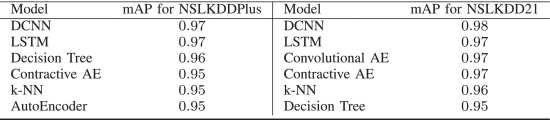
\includegraphics[width=350px]{images/reti_neurali/precisione_media.png}
    \caption{Comparazione precisione media dei metodi di anomaly detection \cite{anomaly_detection_comparativa}.}
    \end{center}
\end{figure}

\begin{figure}[]
    \begin{center}
    \label{fig:anomaly_comparazione_2}
    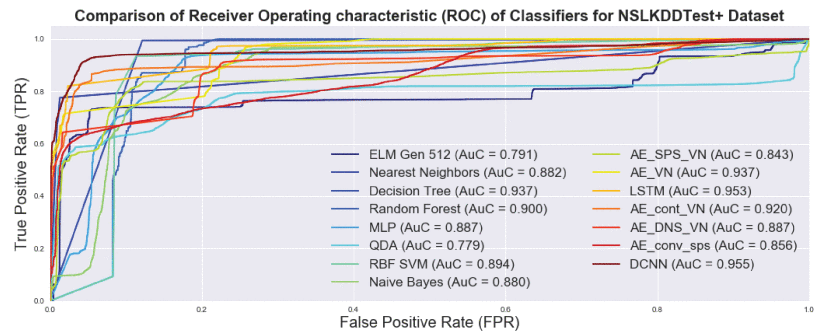
\includegraphics[width=\hsize]{images/reti_neurali/comparazione.png}
    \caption{Comparazione dei metodi di anomaly detection \cite{anomaly_detection_comparativa}.}
    \centering
    \end{center}
\end{figure}


\chapter{Mitigazione degli attacchi}


\section{Introduzione}

Mitigare gli attacchi DDoS è un problema di più difficile risoluzione rispetto alla sola rilevazione, perchè bisogna conoscere maggiori informazioni sulla provenienza del flusso malevolo e il problema dei ``false positive'' è maggiormente sentito: se durante la fase di detection rileviamo un falso positivo e lo notifichiamo all'amministratore di sistema \underline{non è un grande problema} perchè sarà lui ad effettuare una successiva analisi prima di intraprendere azioni correttive. Se ci prefiggiamo l'obiettivo di bloccare automaticamente i flussi malevoli dei falsi positivi significherà degradare la connessione ad utenti legittimi.

\subsection{Ip spoofing}

L'ip spoofing è una tecnica che permette di costruire pacchetti IP con indirizzo IP sorgente modificato con lo scopo di fingersi un altro dispositivo o nascondere la propria identità.È un grande problema di sicurezza delle reti, principalmente perchè permette effettuare attacchi DDoS, permettendo di effettuare attacchi come l'amplificazione DNS oppure rendendo più difficile l'identificazione della sorgente dell'attacco nelle altre tipologie.

%todo: cite https://www.cloudflare.com/it-it/learning/ddos/glossary/ip-spoofing/


\paragraph{Bloccare l'ip spoofing}
Per mitigare questo problema abbiamo introdotto una regola iptables nel router \ref{code:iptablesrule}, la quale impedisce l'inoltro di pacchetti provenienti da sottoreti diverse da quella in cui è situato il router.
Iptables è un firewall integrato nel kernel linux.
% https://wiki.archlinux.org/title/Iptables_(Italiano)#:~:text=Iptables%20%C3%A8%20un%20potente%20firewall,%C3%A8%20usato%20per%20gli%20IPv6.

% todo: la regola è corretta?
\begin{lstlisting}[caption={Esempio di regola iptables}\label{code:iptablesrule}]
    mettere la regola qui
\end{lstlisting}
Questa soluzione impedisce solo parzialmente l'utilizzo dell'ip spoofing, perchè sarà sempre possibile generare pacchetti con ip spoofing provenienti da qualsiasi indirizzo ip della sottorete in cui si trova l'attaccante.


\section{Tool utilizzati}
Prova prova

Per mitigare un attacco devo conoscere un maggior numero di informazioni riguardo al traffico in forma non aggregata, per questa motivazione utilizzo degli ulteriori tool per raccogliere dati sui flussi transitanti per un'interfaccia in maniera non aggregata.

\subsection{Netflow}

Netflow è un software introdotto inizialmente nei router Cisco nel 1996, successivamente è stato creata un'estensione standardizzata dall'IETF, chiamata IPFIX. Netflow è uno dei tool di monitoring più famosi e permette di monitorare e registare informazioni riguardo i flussi che attraversano una determinata interfaccia.
% todo: tabella con features raccolete da netflow

% \begin{center}
%     \begin{tabular}{c c c c c}
%         IN\_BYTES & IN\_PKTS & FLOWS & PROTOCOL & SRC\_TOS \\ TCP\_FLAGS  &  L4\_SRC\_PORT & IPV4\_SRC\_ADDR & SRC\_MASK INPUT\_SNMP \\ L4\_DST\_PORT & IPV4\_DST\_ADDR



%     \end{tabular}
% \end{center}

Poichè non è possibile estendere le features di netflow e non rispecchiano completamente i nostri interessi abbiamo deciso di progettare il nostro agent utilizzando altre soluzioni.
% todo: le features di netflow le posso modificare?

\subsection{Modulo Kernel}

Nella sezione \cite{chapter:our_work} è stata accennata la possibiltà di raccogliere dati con maggiore granularità tramite l'utilizzo di un modulo kernel scritto appositamente.

Nella caso in cui si vogliano aggiungere dei software per collezionare dati maggiormente granulari bisogna intervenire lato kernel, perchè in userspace non esistono meccanismi per analizzare tutti i pacchetti in transito su un'interfaccia. Di conseguenza per aggiungere delle funzioni al kernel Linux esisto solitamente tre soluzioni: la prima è quella di fare aggiungere il codice ufficialmente al suo interno, questa soluzione è la più complicata: sono necessarie le giuste motivazioni per convincere i manteiner ad adottare quella soluzione e inoltre passeranno anni prima della distribuzione in distribuzioni stabili. La seconda è quella di creare un modulo kernel personalizzato, i moduli kernel sono una porzione di codice compilato che possono essere inseriti nel kernel a run-time. Questo metodo è sicuramente più rapido, ma potrebbe portare a vulnerabilità, problemi di compatibilità all'aggiornamento del kernel e rischi di deadlock per l'intero sistema.La terza possibilità è l'uso di eBPF, che esploreremo successivamente.
%Todo: Cercare articolo dove ne parla

La prima versione del nostro software è stata sviluppata scrivendo un modulo kernel che utilizzava netfilter. Questa soluzione è la strada tradizionalmente usata nel mondo Linux e in Tiesse per l'implementazione delle proprie personalizzazioni nei prodotti.
Netfilter è un componente di tutte le moderne distribuzioni Linux, che permette di intercettare e manipolare pacchetti in transito dal router, usato nel kernel permette di registrare delle callback, eseguite alla ricezione di ogni pacchetto su un determinato punto d'aggancio.
Per la scrittura del modulo siamo partiti dalla compilazione del codice sorgente del kernel del router. successivamente è stato scritto un programma in linguaggio C, che sfruttando netfilter aggancia ad un hook, più in particolare ``NF\_INET\_POST\_ROUTING'', una funzione da eseguire alla ricezione di ogni pacchetto, la quale incrementa dei contatori di un vettore.
Terminata la scrittura, il modulo deve essere compilato, nel nostro caso cross compilato per architecture ``arm64''. La compilazione generare un file con estensione .ko e dopo averlo copiato sul router, dovrà essere inserito dinamicamente nel kernel del router tramite il comando ``insmod [nome\_modulo].ko''.

Inoltre in userspace è stato scritto un plugin per collectd, il quale ogni volta che necessita dei dati effettua una lettura su un ``process file system'' (procfs), uno pseudo-filesystem usato per accedere alle informazioni fornite dai processi kernel, tramite il quale il nostro modulo kernel ritorna un JSON con il nome della metrica presa in considerazione e il valore.

Questa soluzione, nonostante fosse la soluzione usata da sempre in azienda, presentava alcuni problemi come la maggior difficoltà di comunicazione tra user-space e kernel-space, la mancanza di strutture dati già esistenti e soprattutto un problema in questo modulo kernel rischiava di portare ad un completo malfunzionamento dell'intero router, per questa ragione abbiamo deciso di adottare una soluzione più moderna.



\begin{figure}[hbtp]
    % todo: capire come gestire citazioni imsmagini a livello di copyright
    %  e capire come funzionano le label per richiamare le immagini
    \label{fig:netfilter}
    \begin{center}
        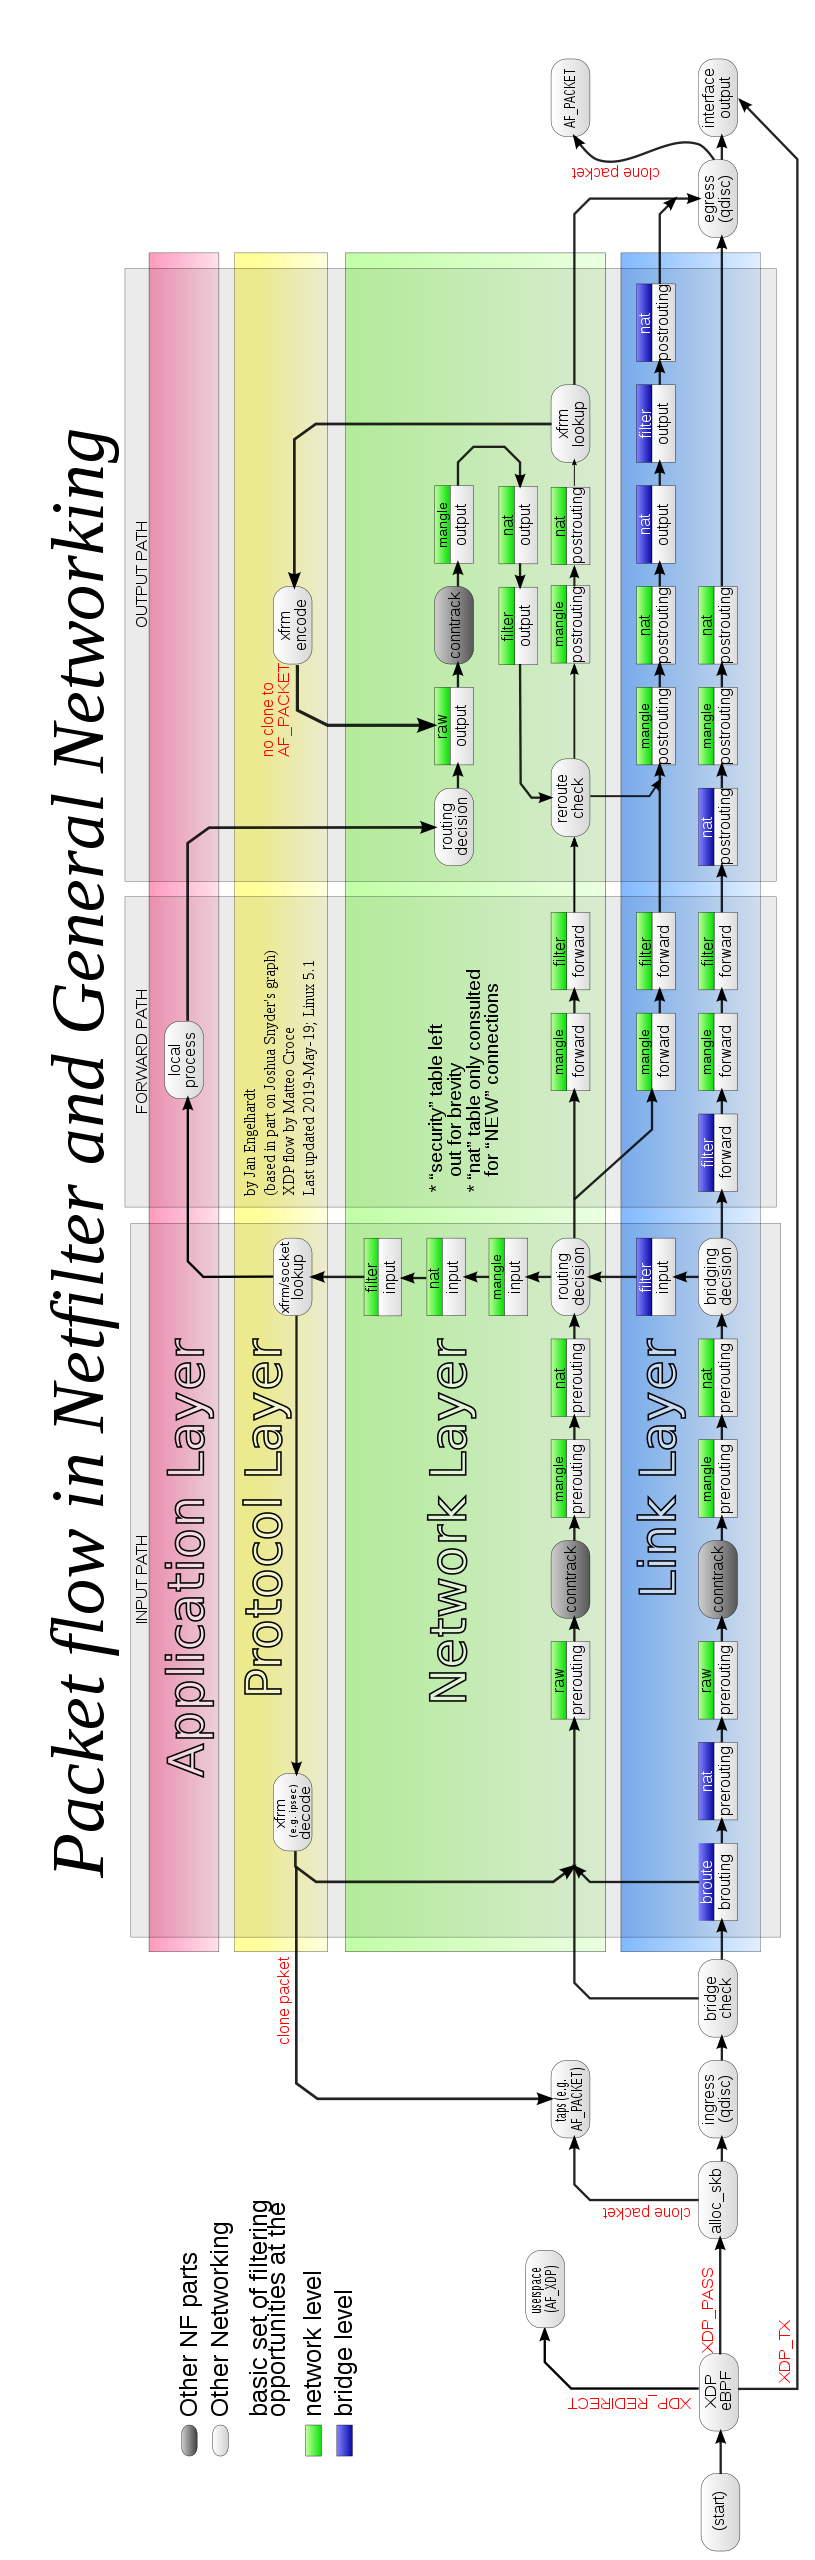
\includegraphics[height=670pt]{images/mitigazione/netfilter.png}
    \end{center}

    \caption{Flusso dei pacchetti in Netfilter}
    \centering
\end{figure}  


\subsection{Berkley Packet Filter (BPF)}

Il Berkley Packet Filter (BPF) è una tecnologia introdotta nel kernel di alcuni sistemi operativi, tra cui il kernel linux, su cui è stata introdotta a partire dalla versione 2.1.75 del kernel, nel 1997. BPF consiste in una macchina virtuale, con una virtual cpu special purpose, integrata nel kernel, che permette il filtraggio e l'analisi dei pacchetti in transito su un'interfaccia.
È una soluzione che permette di eseguire un bytecode in maniera sicura nello spazio kernel utilizzando una sandbox ed eliminando l'overhead delle system call e del context switching tra kernel e user. 
Per effettuare il filtering tramite BPF deve essere generato del codice in un particolare assembly in grado di funzionare sulla CPU virtuale, che verrà richiamato alla ricezione di ogni pacchetto sull'interfaccia determinata (event driven). 
Un esempio del suo utilizzo è tcpdump che sfrutta BPF per effettuare il filtraggio in maniera efficiente. L'esempio di bytecode \ref{code:esempiobpf} permette di filtrare i pacchetti IPV4, per farlo verifica se l'ethertype è uguale a 0x800 \cite{risso_ebpf}.

%todo: cite https://drive.google.com/file/d/14dRWGwAJKBqB1N6-NOBHUxoeOILPYQjN/view
% https://docs.cilium.io/en/stable/bpf/

\begin{lstlisting}[caption={Esempio delle istruzioni per il filtering dei pacchetti IP in BPF assembly}\label{code:esempiobpf}]
user@linux$ tcpdump -d ip
(000) ldh [12]
(001) jeq #0 x800 jt 2 jf 3
(002) ret #96
(003) ret #0
\end{lstlisting}

\subsection{extended Berkeley Packet Filter (eBPF)}
% https://docs.cilium.io/en/stable/bpf/

La extended Berkeley Packet Filter è una versione che estende la versione originale ed è stata introdotta nella versione 3.18 del kernel Linux, ai giorni nostri la versione originale è completamente obsoleta e anche il codice scritto per la vecchia versione, per esempio tcpdump, viene tradotto trasparentemente per la nuova \cite{cilium_ebpf}.

\begin{figure}[]
    \label{fig:ebpf}
    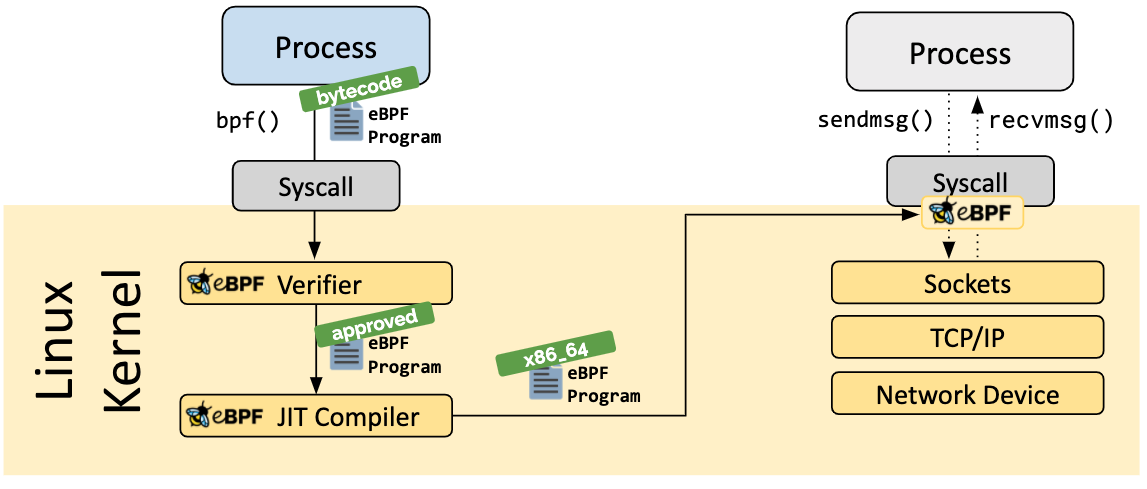
\includegraphics[width=\hsize]{images/mitigazione/ebpf_architecture.png}
    \caption{Architettura eBPF \cite{ebpf.io}.}
    \centering
\end{figure}

Prima che il bytecode sia caricato nel kernel Linux vengono effettuati due passaggi, come si può notare dall'immagine \ref{fig:ebpf}. La prima è la ``Verication'', la quale si occupa di verificare che il programma sia sicuro da eseguire e verifica che: il programma abbia lunghezza limitata, che non ci siano accessi a indirizzi di memoria non validi e che abbia una fine, di conseguenza controlla che non siano presenti cicli infiniti. 
Effettuata la verifica viene eseguita la ``Just-in-Time (JIT) compilation'', la quale traduce il bytecode generico in istruzioni specifiche per la macchina che lo sta eseguendo, questo permette di incrementare le prestazioni e rendere i programmi eBPF efficienti come i moduli kernel compilati nativamente \cite{ebpf.io}.
eBPF inoltre fornisce strumenti utili per lo sviluppo, come le mappe e gli helpers.

Le mappe sono un importante aspetto dei programmi eBPF, esse permettono di memorizzare dati in delle strutture chiave/valore in kernel space, che possono essere condivise con altri programmi eBPF oppure con applicazioni in user space \cite{cilium_ebpf}.

La chiamata di generiche funzioni a livello kernel non è consentita, sia per mantenere la compatibilità del programma non solo con una determinata versione del kernel, per questo motivo sono stati introdotti gli ``helpers'', inoltre permettono l'esecuzione di istruzioni o permettono di eseguire alcuni task non permessi dall'assembly eBPF per motivi di sicurezza.

Un ulteriore caratteristica di eBPF è la possibilità di potere concatenare l'esecuzione dei programmi, chiamandoli a cascata,in maniera simile alla ``execve()'', durante l'esecuzione.

I vantaggi di un programma eBPF rispetto alla scrittura di un modulo kernel sono molteplici: permettono l'esecuzione sicura del codice senza la possibilità che vada a corrompere il kernel, non c'è rischio che le nuovi versioni del kernel vadano a interrompere il suo funzionamento e garantisce le stesse prestazioni.

% https://ebpf.io/

\subsection{eXpress Data Path (XDP)}
\begin{figure}[]
    % todo: capire come gestire citazioni imsmagini a livello di copyright
    % https://www.researchgate.net/publication/333998355_Securing_Linux_with_a_Faster_and_Scalable_Iptables
    \label{fig:hooks}
    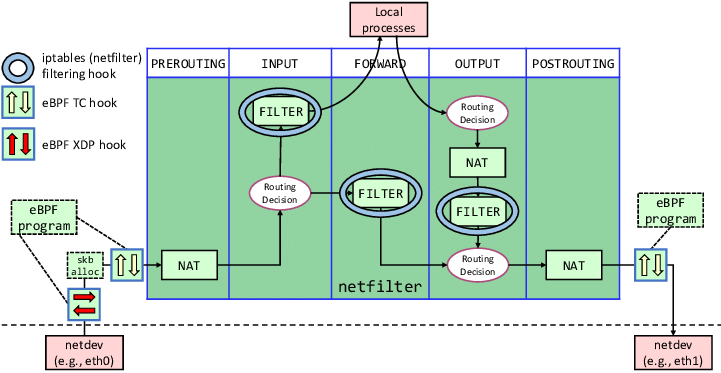
\includegraphics[width=\hsize]{images/mitigazione/hooks.png}
    \caption{Hooks eBPF}
    \centering
\end{figure}
Il kernel Linux supporta più punti dello stack di rete in cui è possibile agganciare l'esecuzione dei programmi eBPF.
XDP (eXpress Data Path) è un hook ad alte performance che permette di eseguire un programma eBPF al primo punto possibile, questo permette grandi performance, perchè il processamento avviene prima che qualsiasi altro processamento possa avvenire. XDP è un punto d'aggancio ideale per il filtering dei pacchetti malevoli o inaspettati e in qualsiasi comune protezione anti DDoS \cite{cilium_xdp}.
Il programma inserito su un hook XDP può compiere cinque azioni possibili:
\begin{itemize}
    \item XDP\_PASS: lascia passare il pacchetto nel normale stack di rete
    \item XDP\_DROP: ignora semplicemente il pacchetto, senza compiere ulteriori azioni
    \item XDP\_TX, restituisce il pacchetto alla stessa interfaccia, normalmente modificato
    \item XDP\_ABORTED: è un valore di ritorno che il programmatore non dovrebbe utilizzare, segnala un che si è verificato un errore nel programma eBPF, per esempio una divisione per zero e contemporaneamente ignora il pacchetto come l'XDP\_DROP
    \item XDP\_REDIRECT: reindirizza il pacchetto verso un'altra scheda di rete, o in user space
\end{itemize}


\subsection{BPF Compiler Collection (BCC)}
 
È un framework che permette la scrittura di programmi python con programmi eBPF incorporati al loro interno. Il framework ha come obiettivo primario i casi in cui eBPF è utilizzata per raccogliere statistiche o compiere azioni in user space al verificarsi di eventi. L'esecuzione del programma eBPF genererà il bytecode che sarà caricato nel kernel \cite{ebpf.io}.
Il programma python potrà comunicare con quello eBPF grazie all'utilizzo delle mappe precedentemente menzionate.

\begin{figure}[]
    % todo: capire come gestire citazioni imsmagini a livello di copyright
    %  e capire come funzionano le label per richiamare le immagini
    \label{fig:bcc}
    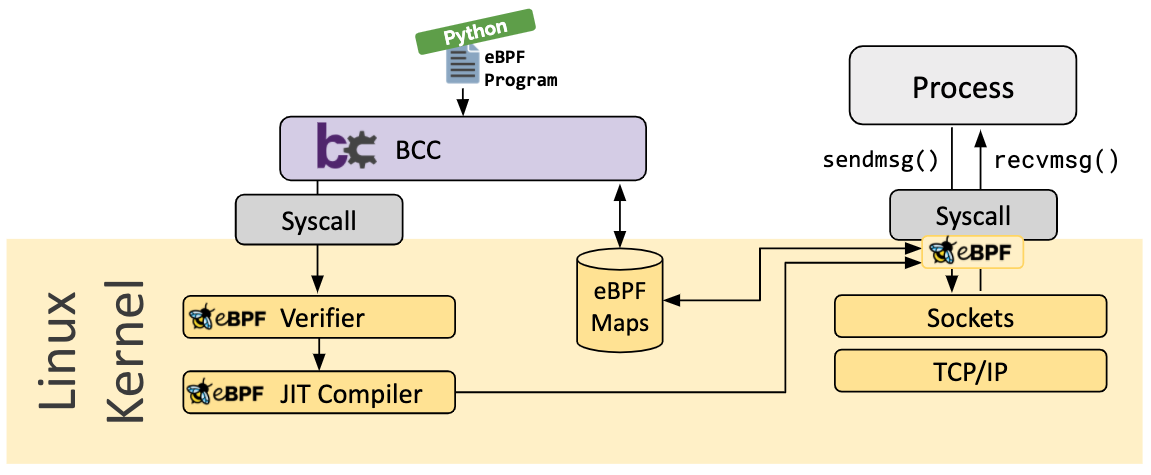
\includegraphics[width=\hsize]{images/mitigazione/bcc.png}
    \caption{Funzionamento di BCC \cite{ebpf.io}}
    \centering
\end{figure}

\section{Funzionamento}

Qua posso parlare di due alternative, la prima è riutilizzare il sistema di anomaly detection simile a quello presentato precedentemente elencando tutti i problemi e i vantaggi.

%todo: citare articoli che usano netflow per rilevare le anomalie

Il secondo consiste nel raccogliere i dati come prima, e creare un ranking per ogni feature risultata anomala precedentemente e a quel punto blocco i flussi sopra una certa soglia, ma quale?

Mentre per l'ip spoofing come la gestisco?

\section{Test sulle anomalie}
\subsection{Tool utilizzati}
\subsection{Risultati}

\chapter{Lavoro futuro}

La soluzione qui sviluppata è stata utilizzata in un ambiente di test, per portare questa applicazione ad uno stato di produzione è necessario introdurre un meccanismo per inviare i segnali tra i molteplici router che hanno comportamento di client e il server più prestazionale che si occupa di calcolare gli anomaly score al verificarsi delle anomalie. Per sviluppare questa comunicazione è possibile utilizzare una connessione TLS diretta tra il client e il server.

Altre funzioni da implementare per ottenere un sistema totalmente funzionante in produzione è un'interfaccia grafica e un sistema di notifiche, tramite i quali l'amministratore di sistema potrà gestire il sistema ed essere allertato in caso di problemi. 

% ma per maggiore comodità in caso in caso di creazione di un'ulteriore interfaccia grafica di amministrazione, potrebbe essere


Per quanto riguarda un'applicazione alternativa di questo sistema di anomaly detection potrebbe essere l'allenare il modello a riconoscere uno specifico pattern di un'applicazione, in modo da potere identificare tale flusso tra tutto il traffico in transito dal router, trasformando l'anomaly score in un "similarity" score.

% todo: lavoro futuro traffico aggregato
Un'altra possibile applicazione futura potrebbe essere aggregare il traffico di tutte le sedi, per avere una panoramica ancora maggiore in caso di attacchi a basso low rate (vedi capitolo x) difficilmente riconoscibili singolarmente.
\chapter{Conclusioni}

Gli attacchi informatici nelle reti business sono sempre più pericolosi a causa della sempre maggiore dipendenza delle aziende dai sistemi informatici, per questo motivo il problema di un singolo distaccamento non deve creare malfunzionamenti all'intera azienda.
% parlo dell'architettura e dei vantaggi dati
Un sistema con filtraggio distribuito come quello da noi proposto permette di non intasare il centro della rete, ma cerca di limitare i problemi direttamente nei CPE.
Inoltre la nostra proposta permette di usare l'infrastruttura già esistente e di essere facilmente modellata per il monitoraggio di servizi specifici, differenti per ogni azienda.
% parlo della scelta del sistema per rilevare gli attacchi, gli attacchi DDoS tendenzialmente creano delle grandi differenze nel traffico dati, per questo motivo abbiamo adottato un meccanismo basato sul riconoscimento delle anomalie.
Lavorando su dei dati aggregati nella prima fase il sistema è in grado di ottenere buoni risultati con un minore utilizzo di risorse rispetto ai sistemi signature-based, i quali devono analizzare ogni flusso e ha il vantaggio di non dovere effettuare aggiornamenti delle regole per riconoscere nuovi attacchi, ma solamente dei nuovi allenamenti del modello in caso di traffico non stazionario. Negli allenamenti della rete successivi al primo si sarà a conoscenza degli intervalli di tempo in cui si sono verificate delle anomalie e se saranno confermate da un amministratore di rete, quei dati potranno essere esclusi e si continuerà a considerarli anomali.
Il sistema mirando al riconoscimento di anomalie generiche potrà essere facilmente esteso per riconoscimento di altre tipologie di attacchi.
Usando gli autoencoder il lavoro necessario per la preparazione del dataset da usare per l'allenamento della rete è incredibilmente ridotto e il risultato ottenuto può essere paragonato ad altri sistemi di anomaly detection che sfruttano altre tecniche.
%  e degli autoencoder, tramite i quali analizziamo informazioni quantitative riguardo al traffico, il sistema è paragonabile ad altri sistemi di anomaly detection. Un sistema di a
Se il traffico generato da un attacco non scatena anomalie, potrà essere facilmente tollerato dalla rete senza creare disservizi.
In presenza di anomalia possiamo decidere il comportamento da tenere in base alla criticità del servizio protetto, ma in ogni caso l'amministratore di rete si troverà molto aiutato nel prendere le decisioni.



\begin{thebibliography}{9}
    \bibitem{ddos_survey_1} Saman Taghavi Zargar, Member, IEEE, James Joshi, Member, IEEE, and David Tipper, Senior Member, IEEE, {\em A Survey of Defense Mechanisms Against Distributed Denial of Service (DDoS) Flooding Attacks}, 2013ss.


    %% da qui va cancellata
    \bibitem{gal} G.~Galilei, {\em Nuovi studii sugli astri medicei}, Manuzio, Venetia, 1612.

    \bibitem{tor1} E.~Torricelli, in ``La pressione barometrica'', {\em Strumenti

            Moderni}, Il Porcellino, Firenze, 1606.
    \bibitem{tor2} E.~Torricelli e A.~Vasari, in ``Delle misure'', {\em Atti Nuovo
            Cimento}, vol.~III, n.~2 (feb. 1607), p.~27--31.

    \bibitem{duane1964} Duane J.T., \emph{Learning Curve Approach To Reliability Monitoring}, IEEE Transactions on Aerospace, Vol. 2, pp. 563-566, 1994

    % altri riferimenti da usare come esempi.

    \bibitem{chiesa2008} Chiesa S., \emph{Affidabilità, sicurezza e manutenzione
        nel progetto dei sistemi}, CLUT, gennaio 2008
    \bibitem{chiesa2}Chiesa S., Fioriti M., Fusaro R., \emph{On Board System
        Technological  Level Improvement Effect on UAV MALE}
    \bibitem{bigliano2010} Bigliano M., \emph{Sicurezza nell'installazione di un velivolo
        senza pilota MALE; applicazione di metodologia di Zonal Safety
        Analysis al velivolo del Progetto SAvE}, Politecnico di Torino,
    maggio 2010
    \bibitem{astrid2012} Chiesa S., Di Meo G.A., Fioriti M., Medici G., Viola N.,
    \emph{ASTRID - Aircraft on board Systems sizing and TRade-off
        analysis in Initial Design}, Research Bulletin, Warsaw University
    of Technology, Institute of Aeronautics and Applied Mechanics,
    p. 1-28, 17-19, ottobre 2012

\end{thebibliography}

% \printbibliography

\end{document}
